 %% LyX 2.3.2 created this file.  For more info, see http://www.lyx.org/.
%% Do not edit unless you really know what you are doing.
\documentclass[12pt,headings=standardclasses]{scrartcl}
\usepackage{amsmath}
\usepackage{amsthm}
\usepackage{mathptmx}
\usepackage{newtxmath}
\renewcommand{\familydefault}{\rmdefault}
\usepackage[T1]{fontenc}
\usepackage[utf8]{inputenc}
\usepackage{geometry}
\geometry{verbose,tmargin=2.5cm,bmargin=2.5cm,lmargin=2.5cm,rmargin=2.5cm}
\usepackage{color}
\usepackage{array}
\usepackage{verbatim}
\usepackage{float}
\usepackage{rotfloat}
\usepackage{booktabs}
\usepackage{bm}
\usepackage{graphicx}
\usepackage{setspace}
\doublespacing

\makeatletter

%%%%%%%%%%%%%%%%%%%%%%%%%%%%%% LyX specific LaTeX commands.
%% Because html converters don't know tabularnewline
\providecommand{\tabularnewline}{\\}

%%%%%%%%%%%%%%%%%%%%%%%%%%%%%% Textclass specific LaTeX commands.
\theoremstyle{plain}
\newtheorem{thm}{\protect\theoremname}[section]
\theoremstyle{plain}
\newtheorem{prop}[thm]{\protect\propositionname}

\@ifundefined{date}{}{\date{}}
%%%%%%%%%%%%%%%%%%%%%%%%%%%%%% User specified LaTeX commands.



\graphicspath{{./figs/}}
\DeclareGraphicsExtensions{.pdf,.jpeg,.png,.eps}
\usepackage{amsthm}
\theoremstyle{definition}
\newtheorem{definition}{Definition}[section]

\usepackage{cleveref}
\usepackage{algorithmic}
\usepackage{array}
\usepackage{stfloats}
\usepackage[super]{nth}
\usepackage{subcaption}
\usepackage{caption}
% for inkscape images
\usepackage{xcolor}
\usepackage{tikz}
\usepackage{pgf}



\g@addto@macro\@floatboxreset\centering


% \usepackage{hyperref}
 
 \AtBeginDocument{% Overrides ref for Cref
 	\let\ref\Cref
 }

\crefalias{prop}{proposition}

% TIKZ
\usepackage{tikz}

% -- Arrows
\usetikzlibrary{arrows}

% --Bayesnet
\usetikzlibrary{bayesnet}
\usetikzlibrary{decorations.pathreplacing}

\tikzset{
	diagonal fill/.style 2 args={fill=#2, path picture={
			\fill[#1, sharp corners] (path picture bounding box.south west) -|
			(path picture bounding box.north east) -- cycle;}},
	reversed diagonal fill/.style 2 args={fill=#2, path picture={
			\fill[#1, sharp corners] (path picture bounding box.north west) |- 
			(path picture bounding box.south east) -- cycle;}}
}

\tikzstyle{partialobs} = [latent,diagonal fill={gray!25}{gray!0}]

%\@ifundefined{showcaptionsetup}{}{%
% \PassOptionsToPackage{caption=false}{subfig}}
%\usepackage{subfig}
%\makeatother

\usepackage[style=chicago-authordate,isbn=false,url=false,eprint=false]{biblatex}
\providecommand{\propositionname}{Proposition}
\providecommand{\theoremname}{Theorem}

\addbibresource{bibliography.bib}
\begin{document}
% INPUT PREAMBLES
% # PAPER SPECIFIC
\global\long\def\Tsq{T^{2}}%
\global\long\def\priordist{p_{z}}%
\global\long\def\detencoding{g_{\mbphi}}%
\global\long\def\detdecoding{f_{\mbtheta}}%
\global\long\def\encoding{q_{\mbphi}(\mbz\g\mbx)}%
\global\long\def\decoding{p_{\mbtheta}(\mbx\g\mbz)}%
\global\long\def\czero{c_{0}}%
\global\long\def\dataset{\mathcal{D}}%
\global\long\def\mbxover#1{\mbx^{(#1)}}%
\global\long\def\stdGauss{\Norm(\mbzero, \mbI)}%
\global\long\def\pdata{p_{data}(x)}%
\global\long\def\ptheta{p_{\mbtheta}}%
\global\long\def\pthetaxgivenz#1#2{\ptheta(#1 \g#2)}%
\global\long\def\qphi{q_{\mbphi}}%
\global\long\def\qphizgivenx#1#2{\qphi(#1 \g#2)}%
\global\long\def\pz{p(\mbz)}%
\global\long\def\oursacronym{SPE}%
\global\long\def\TsqKLD{T_{\mathrm{KLD}}^{2}}%
\global\long\def\QERE{Q_{\mathrm{ERE}}}%
% # TYPOGRAPHY
\global\long\def\etal{\textit{et al}. }%
\global\long\def\ie{\textit{i}.\textit{e}.}%
\global\long\def\eg{\textit{e}.\textit{g}.}%
% # PROBABILITY

\global\long\def\g{\,|\,}%
\global\long\def\gg{\,\|\,}%
\global\long\def\KL#1#2{\textrm{KL}\left(#1\gg#2\right)}%
\global\long\def\E{\mathbb{E}}%
% Expectation

% # DISTRIBUTIONS

\global\long\def\Norm{\mathcal{N}}%
% Gaussian likelihood
\global\long\def\Gam{\textrm{Gam}}%
\global\long\def\InvGam{\textrm{InvGam}}%
% # MISCELLANEOUS

\global\long\def\d#1{\ensuremath{\operatorname{d}\!{#1}}}%
\global\long\def\diag{\textrm{diag}}%
\global\long\def\supp{\textrm{supp}}%
\global\long\def\indep{\mathpalette{\independenT}{\perp}}%
\global\long\def\independenT#1#2{\mathrel{\rlap{$#1#2$}\mkern2mu  {#1#2}}}%
\global\long\def\inv{^{\raisebox{.2ex}{${\scriptscriptstyle -1}$}}}%

% # SET NOTATION
\global\long\def\R{\mathbb{R}}%
% # BOLD MATHEMATICS

\global\long\def\mba{\bm{a}}%
\global\long\def\mbb{\bm{b}}%
\global\long\def\mbc{\bm{c}}%
\global\long\def\mbd{\bm{d}}%
\global\long\def\mbe{\bm{e}}%
%\newcommand{\mbf}{\bm{f}}
\global\long\def\mbg{\bm{g}}%
\global\long\def\mbh{\bm{h}}%
\global\long\def\mbi{\bm{i}}%
\global\long\def\mbj{\bm{j}}%
\global\long\def\mbk{\bm{k}}%
\global\long\def\mbl{\bm{l}}%
\global\long\def\mbm{\bm{m}}%
\global\long\def\mbn{\bm{n}}%
\global\long\def\mbo{\bm{o}}%
\global\long\def\mbp{\bm{p}}%
\global\long\def\mbq{\bm{q}}%
\global\long\def\mbr{\bm{r}}%
\global\long\def\mbs{\bm{s}}%
\global\long\def\mbt{\bm{t}}%
\global\long\def\mbu{\bm{u}}%
\global\long\def\mbv{\bm{v}}%
\global\long\def\mbw{\bm{w}}%
\global\long\def\mbx{\bm{x}}%
\global\long\def\mby{\bm{y}}%
\global\long\def\mbz{\bm{z}}%
\global\long\def\mbA{\bm{A}}%
\global\long\def\mbB{\bm{B}}%
\global\long\def\mbC{\bm{C}}%
\global\long\def\mbD{\bm{D}}%
\global\long\def\mbE{\bm{E}}%
\global\long\def\mbF{\bm{F}}%
\global\long\def\mbG{\bm{G}}%
\global\long\def\mbH{\bm{H}}%
\global\long\def\mbI{\bm{I}}%
\global\long\def\mbJ{\bm{J}}%
\global\long\def\mbK{\bm{K}}%
\global\long\def\mbL{\bm{L}}%
\global\long\def\mbM{\bm{M}}%
\global\long\def\mbN{\bm{N}}%
\global\long\def\mbO{\bm{O}}%
\global\long\def\mbP{\bm{P}}%
\global\long\def\mbQ{\bm{Q}}%
\global\long\def\mbR{\bm{R}}%
\global\long\def\mbS{\bm{S}}%
\global\long\def\mbT{\bm{T}}%
\global\long\def\mbU{\bm{U}}%
\global\long\def\mbV{\bm{V}}%
\global\long\def\mbW{\bm{W}}%
\global\long\def\mbX{\bm{X}}%
\global\long\def\mbY{\bm{Y}}%
\global\long\def\mbZ{\bm{Z}}%
\global\long\def\mbalpha{\bm{\alpha}}%
\global\long\def\mbbeta{\bm{\beta}}%
\global\long\def\mbdelta{\bm{\delta}}%
\global\long\def\mbepsilon{\bm{\epsilon}}%
\global\long\def\mbchi{\bm{\chi}}%
\global\long\def\mbeta{\bm{\eta}}%
\global\long\def\mbgamma{\bm{\gamma}}%
\global\long\def\mbiota{\bm{\iota}}%
\global\long\def\mbkappa{\bm{\kappa}}%
\global\long\def\mblambda{\bm{\lambda}}%
\global\long\def\mbmu{\bm{\mu}}%
\global\long\def\mbnu{\bm{\nu}}%
\global\long\def\mbomega{\bm{\omega}}%
\global\long\def\mbphi{\bm{\phi}}%
\global\long\def\mbpi{\bm{\pi}}%
\global\long\def\mbpsi{\bm{\psi}}%
\global\long\def\mbrho{\bm{\rho}}%
\global\long\def\mbsigma{\bm{\sigma}}%
\global\long\def\mbtau{\bm{\tau}}%
\global\long\def\mbtheta{\bm{\theta}}%
\global\long\def\mbupsilon{\bm{\upsilon}}%
\global\long\def\mbvarepsilon{\bm{\varepsilon}}%
\global\long\def\mbvarphi{\bm{\varphi}}%
\global\long\def\mbvartheta{\bm{\vartheta}}%
\global\long\def\mbvarrho{\bm{\varrho}}%
\global\long\def\mbxi{\bm{\xi}}%
\global\long\def\mbzeta{\bm{\zeta}}%
\global\long\def\mbDelta{\bm{\Delta}}%
\global\long\def\mbGamma{\bm{\Gamma}}%
\global\long\def\mbLambda{\bm{\Lambda}}%
\global\long\def\mbOmega{\bm{\Omega}}%
\global\long\def\mbPhi{\bm{\Phi}}%
\global\long\def\mbPi{\bm{\Pi}}%
\global\long\def\mbPsi{\bm{\Psi}}%
\global\long\def\mbSigma{\bm{\Sigma}}%
\global\long\def\mbTheta{\bm{\Theta}}%
\global\long\def\mbUpsilon{\bm{\Upsilon}}%
\global\long\def\mbXi{\bm{\Xi}}%
\global\long\def\mbzero{\bm{0}}%
\global\long\def\mbone{\bm{1}}%
\global\long\def\mbtwo{\bm{2}}%
\global\long\def\mbthree{\bm{3}}%
\global\long\def\mbfour{\bm{4}}%
\global\long\def\mbfive{\bm{5}}%
\global\long\def\mbsix{\bm{6}}%
\global\long\def\mbseven{\bm{7}}%
\global\long\def\mbeight{\bm{8}}%
\global\long\def\mbnine{\bm{9}}%


\title{Toward a Better Monitoring Statistic for Profile Monitoring with Variational
Autoencoders}
\maketitle
\begin{abstract}
Due to the recent success of deep learning models, nonlinear profile
monitoring schemes based on deep generative models specifically for
variational autoencoders. While these works show impressive results
over classical methods, the proposed monitoring statistic often ignore
shortcomings of learned lower-dimensional representations and computational
limitations of real-world high-dimensional systems. In this work,
we first manifest these issues and then overcome them with a novel
statistic formulation that both increases out-of-control detection
accuracy and computational efficiency. We demonstrate our results
both on a carefully designed simulation study and a real-life example
of image profiles obtained from a hot steel rolling process.

\medskip{}

\textbf{Keywords: }Control charts, deep learning, high-dimensionality,
latent variable modeling, profile monitoring
\end{abstract}

\section{Introduction}

\label{sec:introduction} Profile monitoring has attracted a growing
interest in the literature in the past decades for its ability to
construct control charts with much better representations for certain
types of process measurements\parencite{Woodall2004-bp,Woodall2007-xs,Maleki2018-uo}.
A profile can be defined as a functional relationship between the
response variables and explanatory variables or spatiotemporal coordinates.
In this work, we focus on the case where the profiles generated from
the process are high-dimensional (HD)\textit{\emph{, i.e.}}, the number
of such explanatory variables or spatiotemporal coordinates are large.
Specifically, we focus on sets of HD profiles for which intra-sample
variation lies on a nonlinear low-dimensional manifold \parencite{Shi2016-tg}.
Our motivating example of such HD profiles is presented in \ref{fig:Rolling}
below, in which we exhibit a sample of surface defect image profiles
collected from a hot steel rolling process.

\begin{figure}[H]
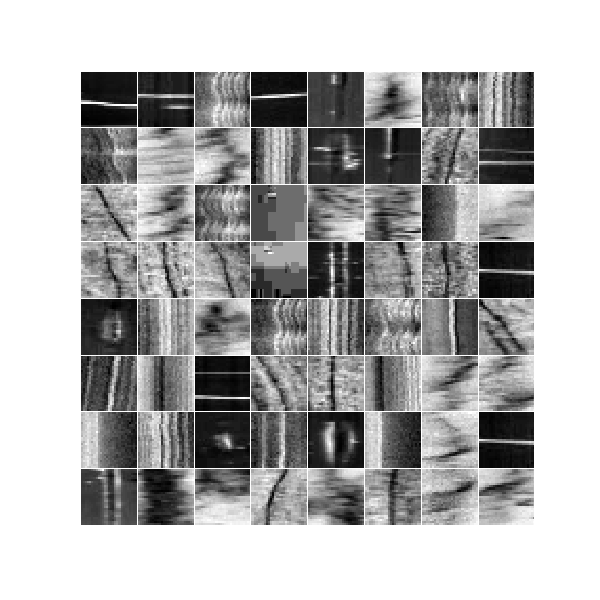
\includegraphics[width=0.5\textheight]{figs/profile_examples} \caption{A collection of 64 by 64 image profiles taken from a hot steel rolling
process.}
\label{fig:Rolling}
\end{figure}

In literature, profile monitoring techniques can be categorized by
their assumptions on the type of functional relationship. Linear profile
monitoring can be considered the most basic profile monitoring technique,
in which it is assumed that the profile can be represented by a linear
function. The idea is to extract the slope and the intercept from
each profile and monitor its coefficients \parencite{zhu2009monitoring}.
Regularization techniques can also be used in linear profile estimation.
For example, \textcite{zou2012lasso} utilizes a multivariate linear
regression model for profiles with the LASSO penalty and use the regression
coefficients for Phase-II monitoring. However, the linearity assumption
can be quite limiting. To address this challenge, nonlinear parametric
models are proposed \parencite{Williams2007-ty,Jensen2009-tu,Noorossana2011-oj,Maleki2018-uo}.
These models assume an explicit family of parameterized functions
and, their parameters are estimated via nonlinear regression. In both
cases, the drawback of both linear and nonlinear parametric models
is that they assume the parametric form is known beforehand, which
might not always be the case.

Another large body of profile monitoring research focuses on the type
of profiles where the basis of the representation is assumed to be
known, but the coefficients are unknown. For instance, to monitor
smooth profiles, various non-parametric methods based on local kernel
regression \parencite{zou2008monitoring,qiu2010nonparametric} and
splines \parencite{chang2010statistical} are developed. To monitor
the non-smooth waveform signals, a wavelet-based mixed effect model
is proposed \parencite{paynabar2011characterization}. However, for
all the aforementioned methods, it is assumed that the nonlinear variation
pattern of the profile is well captured by a known basis or kernel.
Usually, there is no guidance on selecting the right basis of the
representation for the original data and it normally requires many
trial and error.

In the case that the basis of HD profiles are not known, dimensionality
reduction techniques are widely used. Principal component analysis
(PCA) is arguably the most popular method in this context for profile
data monitoring because of its simplicity, scalability, and good data
compression capability. In \textcite{liu1995control}, PCA is proposed
to reduce the dimensionality of the streaming data and, $T^{2}$ and
$Q$ charts are constructed to monitor the extracted representations
and residuals, respectively. To generalize PCA methods to monitor
the complex correlation among the channels of multi-channel profiles,
\textcite{paynabar2015change} propose a multivariate functional PCA
method and apply change point detection methods on the function coefficients.
Along this line, tensor-based PCA methods are also proposed for multi-channel
profiles, examples including uncorrelated multi-linear PCA \parencite{paynabar2013monitoring}
and multi-linear PCA \parencite{grasso2014profile}. Finally, various
tensor-based PCA methods \parencite{yan2015image} are compared and
different test statistics are developed for tensor-based process monitoring.

The main limitation of all the aforementioned PCA-related methods
is that the expressive power of linear transformations is very limited.
Furthermore, each principal component represents a global variation
pattern of the original profiles, which is not efficient at capturing
the local spatial correlation within a single profile. Therefore,
PCA requires much larger latent space dimensions than the dimension
of the actual latent space, yielding a sub-optimal and overfitting-prone
representation. This phenomenon hinders profile monitoring performance.

A systematic discussion of this issue is articulated in \parencite{Shi2016-tg}.
In that work, the authors identify the problems associated with assuming
a closeness relationship in the subspace that is characterized by
Euclidean metrics. They successfully observe that the intra-sample
variation in complex high-dimensional corpora may lie on a nonlinear
manifold as opposed to a linear manifold, which is assumed by PCA
and related methods. However, the authors only focus on applying manifold
learning for Phase-I analysis, while the Phase-II monitoring procedure
is not touched upon.

Deep dimensionality reduction models have been proposed as an alternative
to classical dimensionality reduction techniques in a handful. Deep
autoencoders have been proposed for profile monitoring for Phase-I
analysis in \parencite{Howard2018-op}. \textcite{Yan2016-wa} compared
the performance of contractive autoencoders and denoising autoencoders
for Phase-II monitoring. \textcite{Zhang2018-js} proposed a denoising
autoencoder for process monitoring. Aside from deterministic deep
neural networks, only three works \parencite{wang2019systematic,Zhang2019-lu,lee2019process}
proposed to use deep probabilistic latent variable models, specifically,
variational autoencoders (VAE), for Phase-II monitoring. All the monitoring statistics in those works differ slightly, but
they are all extensions of the classic $T^{2}$ and $Q$-charts of
PCA. We argue that there is room for improvement for the monitoring
statistic formulations in those works for several reasons, especially
when high-dimensional profiles are considered. In this work, we propose
a new monitoring statistic formulation to address this issue.

The contributions of this work are as follows:
\begin{itemize}
\item We compare all the existing monitoring statistics for deep latent
variable models with the focus on the VAE model and propose a better
monitoring statistic that responds robustly and, in most cases, more
accurately than previous formulations requiring only a single pass
through the autoencoder.
\item We give insight into the existing monitoring statistics for latent-variable
models with a focus on variational autoencoders and classify them
based on the latent-variable based and residual-based monitoring statistics.
We also show how these statistics are natural extensions to the monitoring
statistics for traditional dimension reduction methods such as probabilistic
PCA.
\item Unlike traditional monitoring statistics for PCA,
we demonstrate through extensive experiments and give insight on why latent variable-based monitoring
statistics should not be used due to the two issues related to deep
neural network encoders: 1) their representations are likely entangled
2) they will likely fail to extrapolate well beyond the region of
in-control profiles.
\item We derive two approximations on the residual-based monitoring statistics
leveraging on the first-order and second-order Taylor expansion and
compare with the sampling-based monitoring statistics. We have demonstrated
that the first-order approximation of the residual-based monitoring
statistics gives the best overall detection accuracy and is computationally
efficient.
\item We demonstrate the effectiveness of this new formulation on both simulation
and real-life case studies and conclude that residual-based monitoring
statistics with deep learning architecture as encoders and decoders
outperform other monitoring statistics and the traditional non-deep-learning-based
methods.
\end{itemize}
%
The rest of the paper is organized as follows: \ref{sec:Background}
first introduces variational autoencoders and reviews traditional
$T^{2}$ and $Q$ charts of PCA as well as the existing monitoring
statistics for VAE. \ref{sec:methodology} introduces the proposed
monitoring statistic and gives insights on its meaning and mathematical
relationship with the traditional PCA methods. \ref{sec:Simulation-Study-Analysis}
shows the simulation study to demonstrate the performance of the proposed
method and give insight into why only the residual-based statistics
is recommended and how to make sure it is computationally efficient.
Finally, \ref{sec:case-study} demonstrates the advantages of the
proposed methodology on a real-life case study,
using images from hot-steel rolling processes.

\section{Background \label{sec:Background}}

\subsection{Variational Autoencoders \label{sec:bckgrnd:lvms}}

In this section, we introduce Variational Autoencoder (VAE) \parencite{Kingma2013-dl},
which is the primary modeling tool in this work. The Gaussian factorized
latent variable model perspective of VAEs is crucial to understand
the role of this model in the context of profile monitoring. This
is why we begin with an introduction to latent variable modeling.

Latent variables models are powerful tools to model complex distributions
over high-dimen\-sional spaces. The underlying assumption is that there
exists a low-dimensional latent structure that explains well the variations
in the high-dimensional observed space. Typically, the density over
observed variables can be decoupled into the distribution on the latent
variables $\pz$ and the conditional distribution of observed variables
given latent variables $p(\mbx\g\mbz)$. Then, these distributions
can be assigned to tractable families of distributions, such as Gaussian.
This enables a more efficient modeling of the data distribution $p(\mbx)$.

A typical example of latent variable models is when the joint distribution
is Gaussian factorized as in \ref{eq:gaussian-factorized}. 
\begin{equation}
\begin{split}\pz & =\Norm(\mbz;0,\mbI_{r})\\
\decoding & =\Norm(\mbx;\mu_{\mbtheta}(\mbz),\sigma^{2}\mbI_{d})\\
p_{\mbtheta}(\mbx,\mbz) & =\decoding\pz
\end{split}
\label{eq:gaussian-factorized}
\end{equation}
In the above formulation, $\mbx\in\R^{d}$ are observed samples, and
$\mbz\in\R^{r}$ are latent variables while $\mu_{\mbtheta}\colon\R^{r}\to\R^{d}$
is a function parameterized by $\mbtheta\in\Theta$, which describes
the relationship between the latent variables and the mean of the
conditional distribution. The Gaussian prior $\pz$ is typically chosen
to be standard multivariate Gaussian distribution to avoid degenerate
solutions \parencite{roweis1999unifying} and conditional covariance
is typically assumed to be isotropic $\sigma^{2}I_{d}$ to avoid ill-defined
problems. The aim is to approximate the true density $p_{\mbtheta}(\mbx)\approx p(\mbx)$
and this approximation can be obtained through marginalization: 
\[
p_{\mbtheta}(\mbx)=\int p_{\mbtheta}(\mbx,\mbz)d\mbz
\]
Finally, in literature, there have been discussions about whether
the independent latent structure assumption $\pz=\Norm(\mbz;0,\mbI_{r})$
can lead to the discovery of the true disentangled variations, a task
also known as disentangled representation learning \parencite[Sec. 3.5]{bengio2013representation}.
Disentangled representations are useful to represent variations in
latent variations due to their ability to separate the independent
factors. However, a discussion on what disentangled representation
implies for profile monitoring is necessary. We are interested in
whether and if so, how such representations will be critical for profile
monitoring.

A famous member of the family of models described above is the probabilistic
principal component analysis (PPCA) \parencite{tipping1999probabilistic}.
The parameters are optimized via a maximum likelihood estimation framework
and it can be solved analytically since $\mu_{\mbtheta}$ is a simple
linear transformation. This enables reusing analytical results from
solutions to the classical PCA problem. The assumption of PPCA that
the latent and observed variables have a strictly linear relationship
is restrictive. In real-world processes, it is likely that this relationship
is highly nonlinear. Deep latent variable models are a marriage of
deep neural networks and latent variable models that aim to solve
this problem. Deep learning has enjoyed a tremendous resurgence in
the last decade due to their superior performance that was unprecedented
for many tasks such as image classification \parencite{krizhevsky2012imagenet},
machine translation \parencite{bahdanau2014neural}, and speech recognition
\parencite{amodei2016deep}. In theory, under sufficient conditions,
a two-layer multilayer perceptron can approximate any function on
a bounded region \parencite{cybenko1989approximation,Hornik1991-li}.
However, growing the width of shallow networks exponentially
for arbitrarily complex tasks is not practical. It has been shown
that deeper representations can often achieve better expressive power
than shallow networks with fewer parameters due to the efficient reuse
of the previous layers \parencite{eldan2016power}.

VAE is arguably the most foundational member of the deep latent variable
model family. The main difference between PPCA and VAE is that VAE
replaces the linear transformation with a high-capacity deep neural
network (called \textit{generative} or \textit{decoder}). This is
powerful in the sense that, along with a general-purpose prior $\pz$,
deep neural networks can transfer such prior to model a wide variety
of densities to model the training data \parencite{kingma2019introduction}.
Unlike PPCA, these models will not have analytical solutions due to
the complex nature of the neural network used. Like most other deep
learning models, their parameters have to be optimized via gradient
descent for maximum likelihood. The problem becomes even harder given
the observation that the posterior $\decoding$ takes meaningful values
only for a small sub-region within $\R^{r}$. This makes sampling
from the prior $\pz$ to estimate the likelihood prohibitively expensive.
Both models work around this problem using the importance sampling
framework \parencite[532]{bishop2006pattern}, where they introduce
another network (called \textit{recognition} or \textit{encoder})
to approximate a proposal distribution $\encoding$ ---parametrized
by $\mbphi$--- which will hopefully sample latent variables from
a much smaller region that is more likely to produce higher posterior
densities for a given input $\mbx$. In fact, PPCA can be treated
as a special case of VAE, where the decoder is modeled by linear transformation.

One important output of a trained VAE is the likelihood estimator.
Once the two networks are trained, the log-likelihood $\log\ptheta(\mbx)$
can be approximated by a Monte Carlo sampling procedure with $L$
iterations \parencite[30]{kingma2019introduction}: 
\begin{equation}
\log\ptheta(\mbx)\approx\log\frac{1}{L}\sum_{l=1}^{L}\frac{\ptheta(\mbx,\mbz^{(l)})}{\qphizgivenx{\mbz^{(l)}}{\mbx}}\label{eqn:SummationLL}
\end{equation}

VAEs are trained to maximize the so-called evidence lower bound (ELBO),
which is deemed a proxy to the likelihood: 
\begin{equation}
\begin{split}\text{ELBO} & \triangleq\log\left(p(\mbx)\right)-\KL{\encoding}{q^{*}(\mbz|\mbx)}\\
 & =\E_{\mbz\sim q_{\mbtheta}}\log\decoding+\KL{\encoding}{p(\mbz)}
\end{split}
\label{eqn:VAELoss}
\end{equation}
where $\KL{\cdot}{\cdot}$ denotes the Kullback-Leibler divergence
(KLD) between two distributions. The left-hand side is the quantity
of interest, while the right-hand side is the tractable expression
that guides the updating of parameters $\mbtheta,\mbphi$ in an end-to-end
fashion.

\subsection{Review of $\protect\Tsq$ and $Q$ Statistics in PCA}

\label{sec:bckgrnd:ReviewPCA} Process monitoring via PCA is typically
undertaken using the $\Tsq$ and $Q$ statistics \parencite{Chen2004-px}.
The $Q$ statistic for PCA is defined as the reconstruction error
between the real sample $\mbx$ and the reconstructed sample $\tilde{\mbx}$.
Its geometric representation is how far the sample is away from the
learned subspace of in-control samples. $\Tsq$ represents how far
the latent representation of that sample is away from the cluster
of latent codes of the in-control samples.

The $\Tsq$ statistics and $Q$ statistic for PCA are defined as follows:
\begin{equation}
\begin{split}Q(\mbx) & =\gg\mbx-\tilde{\mbx}\gg^{2}\\
\Tsq_{PCA}(\mbx) & =\mbz^{\top}\mbSigma\inv_{r}\mbz=\mbx^{\top}\mbW_{r}\mbSigma\inv_{r}\mbW_{r}^{\top}\mbx,
\end{split}
\label{eqn: QTPCA}
\end{equation}
where matrix $\mbW_{r}$ is the loading matrix, and $\mbSigma\inv_{r}$
is the inverse of the covariance matrix when only the first $r$ principal
components are kept. There are various methods to choose $r$ such
as fixing the percentage of variation explained \parencite[41]{Chiang2001-nu}.

For processes with relatively small latent and residual dimensionality,
the upper control limits of these statistics for the $\alpha$\% Type-1
error tolerance is constructed by employing the normality assumptions
of PPCA \parencite[43-44]{Chiang2001-nu}. However, using such measures
for high-dimensional nonlinear profiles is prohibitively error-prone
as both $r$ and $d$ will be much higher than the assumptions on
chi-square distribution can tolerate. As an alternative, non-parametric
methods to estimate upper percentiles are increasingly used for this
purpose, such as simple sample percentile on a held-out set (i.e.,
validation set) or fitting kernel density estimation to in-control
statistics.

\subsection{Review and Critique of Previously Proposed Monitoring Statistics
Proposed for VAE}

\label{sec:bckgrnd:critique} Three works have recently considered
VAE for process monitoring, all of which propose different statistic
formulations for monitoring. \textcite{Zhang2019-lu} proposed to
use only $H^{2}$ for the process monitoring, which is basically the
Mahalanobis distance of the mean of the proposal distribution from
standard Gaussian distribution. 
\begin{equation}
H^{2}=\mu_{\mbphi}(\mbx)^{\top}\mu_{\mbphi}(\mbx)
\end{equation}
The major drawback of using only this statistic is that it completely
ignores the disturbances in residual distribution.

\textcite{lee2019process} claimed to use $T^{2}$ and $Q$ of PCA
for VAE. For a given input $\mbx$, a single sample is drawn from
the proposal distribution $\mbz^{(l)}\sim\encoding$ which is used
reconstruct the input using the generative model $\mbx^{(l)}\sim p_{\mbtheta}(\mbx\g\mbz^{(l)})$.
The proposed test statistics in this work are as follows: 
\begin{equation}
\begin{aligned}T^{2} & =(\mbz^{(l)}-\bar{\mbz})^{\top}S_{\mbz}\inv(\mbz^{(l)}-\bar{\mbz})\\
SPE & =\gg\mbx^{(l)}-\mbx\gg_{2}^{2},
\end{aligned}
\end{equation}
where $\bar{\mbz}$ and $S_{\mbz}\inv$ are estimated over a single
loop from the data. The proposed control charting methodology suggested
that these two statistics work in combination and at least one vote
of either statistics is enough to make a detection decision. However,
the estimation of the $\bar{\mbz}$ and $S_{\mbz}\inv$ can be slow
and unnecessary since for a well-trained VAE, $\bar{\mbz}$ and $S_{\mbz}\inv$
would be approximately equal to 0 and $I$, respectively. Instead,
the estimation can be unstable when data is limited.

Finally, \textcite{wang2019systematic} proposed the $R$ and $D$
statistics by focusing on the two major components of the tractable
part of the objective function of VAE shown as in \ref{eqn:VAELoss}.
The $D$ statistic is simply the KL divergence between the prior and
proposal. For $R$ statistic, like \textcite{lee2019process}, they
employ summary statistics over samples from proposal but also claim
that sampling size can be fixed to one: 
\begin{equation}
\begin{aligned}D & =\KL{\encoding}{p(\mbz)}\\
R & =\frac{1}{L}\sum_{l=1}^{L}-\log q_{\mbtheta}(\mbx\g\mbz^{(l)}),
\end{aligned}
\label{eq: DR}
\end{equation}
$SPE$ in and $R$ are essentially the same quantities up to a constant,
which makes them identical in the context of monitoring statistics.
This is why we will refer to them as $SPE/R$ throughout the rest
of the paper.

\section{Methodology}

\label{sec:methodology}

\subsection{Proposed Monitoring Statistic}

\label{sec:proposed-statistic}

Log-likelihood, $\log\ptheta(\mbx)$, arises as a natural monitoring
statistic candidate in the context of VAEs. That is, given a well-trained VAE, in-control samples should have relatively larger log-likelihood
than out-of-control samples. However, the required number of Monte
Carlo samples---$L$ in \ref{eqn:SummationLL}--- can be prohibitively
large to get meaningful estimates of the likelihood \parencite{Kingma2013-dl}.
This will make it intractable to monitor high throughput systems in
real-time. To address this issue, ELBO defined in \ref{eqn:VAELoss}
can be used for a reasonable approximation:

\begin{equation}
\E_{\mbz\sim q_{\mbtheta}}\log\decoding+\KL{\encoding}{p(\mbz)}\label{eqn: VAEELBO}
\end{equation}

A natural tendency in the literature is to break ELBO
into two terms: $\E_{\mbz\sim q_{\mbtheta}}\log\decoding$ and $\KL{\encoding}{p(\mbz)}$.
To understand the role of these two terms in process monitoring, we
revisit the assumptions of the model described in \ref{eq:gaussian-factorized}.
Let us formally represent an out-of-control distribution as $p_{\delta}(\mbx)\neq p(\mbx)$.
Since $p(\mbx)=\int p(\mbx\g\mbz)p(\mbz)d\mbz$, we can observe two
sources of out-of-control behaviors: disturbances in latent distribution
$p_{\delta}(\mbz)\neq\pz$ and disturbances in residual distribution
$p_{\delta}(\mbx\g\mbz)\neq p(\mbx\g\mbz)$. Note that various combinations
of these two disturbances cover disturbances in the entire process.
One can argue that $\E_{\mbz\sim q_{\mbtheta}}\log\decoding$ can
detect the disturbances in the residual space $p_{\delta}(\mbx\g\mbz)\neq p(\mbx\g\mbz)$
and $\KL{\encoding}{p(\mbz)}$ can detect the disturbance in the latent
space $p_{\delta}(\mbz)\neq\pz$. This is actually true for linear
latent variable models. Since we know that for simpler data that can
be accurately modeled by PCA, both terms play an important role \parencite{kim2003process}
for process monitoring. This also holds for PPCA and will become the
$T^{2}$ and $Q$ statistics in the traditional monitoring framework.
To prove this, we link the $T^{2}$ and $Q$ statistics of PPCA
(see \ref{sec:bckgrnd:ReviewPCA}) using the ELBO framework.
\begin{prop}
\label{prop: T2Q} We know from the definition of PPCA \parencite{tipping1999probabilistic}
that the prior, encoding and decoding functions are normally distributed
as: 
\[
\begin{split}p(\mbz) & =\Norm(0,\mbI),\\
\decoding & =\Norm(\mbW\mbz,\sigma^{2}\mbI).\label{eq:Gaussian}
\end{split}
\]
In this case, from PPCA, the encoder can be solved analytically as
another normal distribution as $\encoding=\Norm(\mu_{\mbphi}(\mbx),\Sigma_{z})$,
where $\mu_{\mbphi}(\mbx)=\mbM^{-1}\mbW^{\top}\mbx$, $\Sigma_{z}=\sigma^{2}\mbM^{-1}$,
and $\mbM=\mbW^{\top}\mbW+\sigma^{2}\mbI$. Then, the two monitoring
statistics defined in \ref{eqn: VAEELBO} can be derived as: 
\begin{equation}
\KL{\encoding}{p(\mbz)}=\frac{1}{2}\gg\mu_{\mbphi}(\mbx)\gg^{2}+C_{1},\label{eqn:KL_PPCA}
\end{equation}
\begin{equation}
\E_{\mbz\sim q_{\mbphi}}\log\decoding\propto\gg\mbx-\mbW\mu_{\mbphi}(\mbx)\gg^{2}+C_{2},\label{eqn:E_PPCA}
\end{equation}
where $C_{1}$ and $C_{2}$ are constants that doesn't depend on $x$.
\end{prop}

The proof is given in \ref{sec:PoofOfPropTQ}. Note that the constants
do not affect the profile monitoring decision. Thus, the test statistics
$\KL{\encoding}{p(\mbz)}$ is equivalent to the $T^{2}$ Statistics
of PCA as defined in \ref{eqn: QTPCA}, and $\E_{\mbz\sim q_{\mbphi}}\log\decoding$
is equivalent the $Q$ statistic in the PCA case. Observe that previously
proposed formulations mentioned in \ref{sec:bckgrnd:critique} rely---directly
or indirectly---on this framework. Statistics $R$ and $SPE$ are
based on $Q$ or in the case of PPCA $\E_{\mbz\sim q_{\mbphi}}\log\decoding$.
Let us call these \emph{residual-based statistics}. The statistics
$H^{2},T^{2}$ and $D$ are based on $T^{2}$ of PCA or $\KL{\encoding}{p(\mbz)}$
of PPCA. We call these \emph{latent-variable based statistics}, as
they rely exclusively on latent representations.

Our first major claim is that latent variable-based statistics are
not useful for profile monitoring when deep neural network based encoders
are used to produce latent representations with the following reasons:
\begin{enumerate}
\item In high-dimensional complex processes, most of the change or disturbances
should be expected on residual distribution. According to \textcite{severson2016perspectives}
faults in complex real-life processes tend to alter the existing relationship
between latent sources of variation as opposed to pushing to most
extreme cases in the latent variational sources. This effect is amplified
for the deep autoencoders since it typically requires a much smaller
latent dimension compared to PCA, due to better data compression capabilities
compared to the traditional PCA methods. This leaves a much smaller
chance for change happening in the latent space.
\item The mean encoder $\mu_{\mbphi}$---modeled by the deep neural network---is
likely to lack two important features: disentangled representations
and extrapolation capabilities. These two qualities are required so
that extreme values of latent variables consistently converge out
of the in-control zone. We illustrate this in \ref{fig:entang-extrap}
below. Observe how Point C is falsely identified as in-control when
learned representations are not disentangled or when they fail to
extrapolate.
\end{enumerate}
\begin{figure}[H]
\begin{centering}
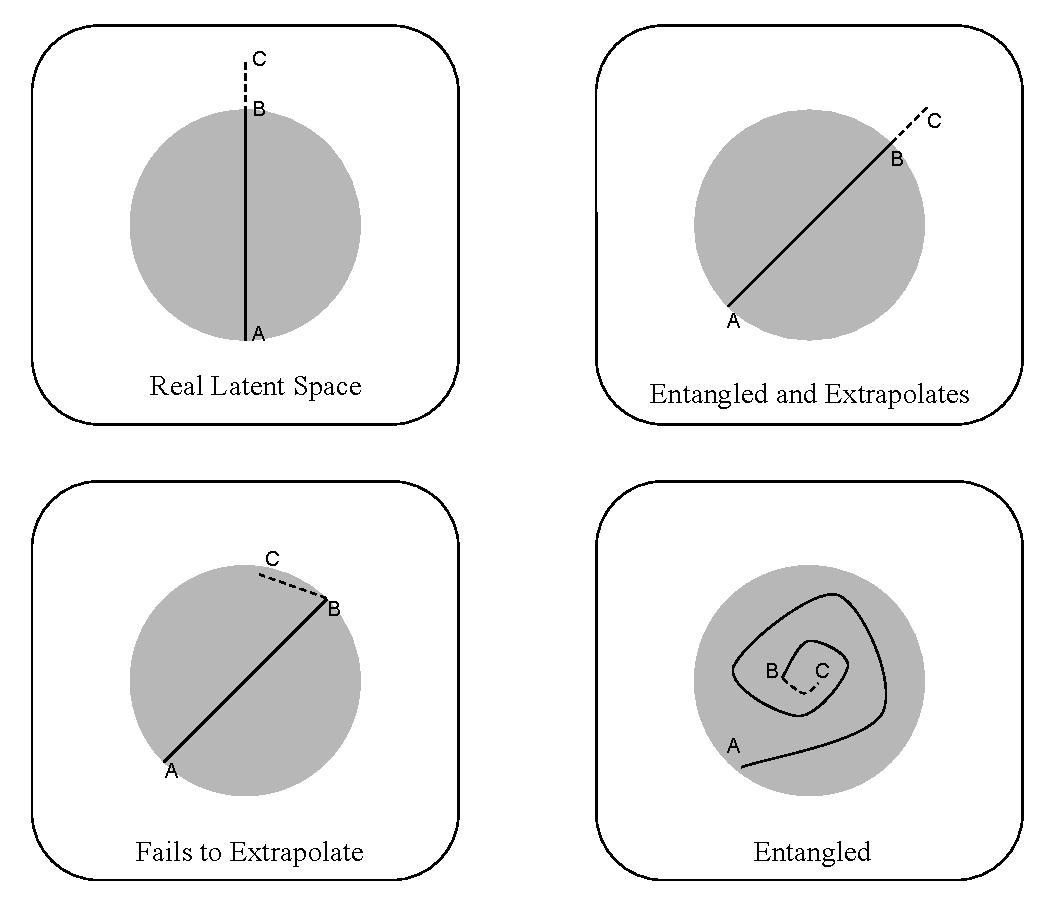
\includegraphics[width=0.9\textwidth]{figs/Disentangled_Extrapolated}
\par\end{centering}
\caption{Different failure mode possibilities of learned two-dimensional latent
space representation of the independent source of variation. \textbf{Top:}
A hypothetical in-control latent space (gray area) and a range of
the independent source of variation (ABC line). Points A and B are
extreme values of in-control range and point C denotes an out-of-control
sample. \textbf{Bottom Left:} A learned representation that fails
to extrapolate. \textbf{Bottom Right:} A learned representation that
is entangled (i.e., not axis-parallel). \label{fig:entang-extrap}}
\end{figure}

Theorem 1 in \textcite{locatello2018challenging} proved that without
proper inductive biases injected into the model about sources of variation,
it is impossible to find disentangled representations. Unfortunately,
injecting such inductive biases requires unrealistically accurate
anticipation of variations among in-control samples as well as specialized
neural network structures, both of which are extremely challenging
tasks given the potential complexity of the processes that generate
high-dimensional profiles. Moreover, even if the representations are
disentangled, correct mappings of $\encoding$ may still not be obtained
outside the training regions due to the failure to extrapolate. Deep
neural networks approximate well only at a bounded domain defined
by where the training set---in our case, the in-control set---is
densely sampled from. The behavior of the function is often unpredictable
outside the training domain. In other words, it may not extrapolate
well beyond the domain of training samples. We refer interested readers
to \ref{app:rosenbrock}, where we replicated this phenomenon on a
toy example. To see why this is a problem, first note that the encoder
$\encoding$ will only be trained with profiles densely sampled from
the bounded region of in-control samples, for which $\pz$ are high.
The behavior of the encoder is uncertain for profiles coming from
dense regions of the out-of-control latent structure $p_{\delta}(\mbz)\neq\pz$.
We expect increased false negatives should the model falsely map these
profiles onto high-density regions of $\pz$ but not $p_{\delta}(\mbz)$.

Unlike latent variable-based statistics, extrapolation issues in $\decoding$
and $\encoding$ actually help the residual-based statistic detect
faults better. We will see this in two cases: 1) if the change happens
in the residual space, $p_{\delta}(\mbx\g\mbz)\neq p(\mbx\g\mbz)$,
it is clear that the residual-based statistics $\E_{\mbz\sim q_{\mbtheta}}\log\decoding$
will be effective at capturing this. 2) More interestingly, this holds
true even when the disturbance is purely on the latent structure $p_{\delta}(\mbz)\neq p(z)$.
This is true no matter if the encoder can correctly map $\encoding$
the out-of-control sample $\boldsymbol{x}^{oc}$ into the in-control
region $\pz$. a) if the encoder $\encoding$ map the out-of-control
sample $\boldsymbol{x}$ into the latent space $\boldsymbol{z}$ in
the in-control domain (i.e., $\pz$), this will lead to the increase
of the monitoring statistics based on the residual space for better
detection power. b) even if the mapping was correct and it maps $\boldsymbol{z}$
outside the in-control region (i.e., $p_{\delta}(\mbz)$), the decoder
$\decoding$ have not been trained for any $\boldsymbol{z}$ outside
$p(z)$, which still leads to a large statistics to capture disturbances
in latent variations. In conclusion, we will recommend using the residual-based
monitoring statistics for both types of changes.

As of now, we have justified the reasons to recommend the use of residual-based
statistics as the only type of test statistics for the profile monitoring
application that uses deep autoencoders such as VAE. Indeed, variations
of the residual-based statistics have been previously proposed in
the literature: $SPE$ of \textcite{lee2019process} and $R$ \textcite{wang2019systematic}.
However, they both use random samples from the proposal distribution
to estimate the expectation. This approach may require a large number
of samples to be generated, and thus a large number of the forward
passes on the decoder network, which is prohibitively expensive in
terms of computation. Instead, we propose a Taylor expansion based
approximation as the proposed statistic. First, observe that $\log\decoding\propto\gg x-\mbmu_{\mbtheta}(z)\gg_{2}^{2}+C$
for all $\mbx$ and $\mbz$ because of the common isotropic covariance
assumption. The constant $C$ can be discarded as noneffective in
terms of control charting because it would only translate the limits
and the statistics by the same amount for any given $\mbx$ and $\mbz$.
We can define $\E_{\mbz\sim q_{\phi}}\gg x-\mbmu_{\mbtheta}(z)\gg_{2}^{2}$
as the expected reconstruction error (ERE) We argue that, the Taylor
expansion for the first-order and second-order moment of the ERE $\E_{\mbz\sim q_{\phi}}\gg x-\mbmu_{\mbtheta}(z)\gg_{2}^{2}$
given the random variable $\mbz\sim\encoding$ can be derived analytically
as follows.
\begin{prop}
The first and second-order Taylor Expansion (denoted by $ERE_{1}$
and $ERE_{2}$ respectively) for the function $\E_{\mbz\sim q_{\phi}}\gg x-\mbmu_{\mbtheta}(z)\gg_{2}^{2}$
given the random variable $\mbz\sim\encoding$ where $\decoding=\Norm(\mu_{\mbphi}(\mbx),\diag(\mbsigma_{\mbphi}(x)))$
can be derived analytically as:
\begin{equation}
ERE_{1}=\gg\mbx-\mbmu_{\mbtheta}(\mbmu_{\mbphi}(\mbx))\gg_{2}^{2}\label{eq:ere-1}
\end{equation}

\begin{equation}
ERE_{2}=\gg\mbx-\mbmu_{\mbtheta}(\mbmu_{\mbphi}(\mbx))\gg_{2}^{2}+\frac{1}{2}\mathrm{tr}(\mathbf{H}_{z}\diag(\mbsigma_{\mbphi}(x)))\label{eq:ere-2}
\end{equation}
where $\mathbf{H}_{z}$ is the Hessian of the function $\gg x-\mbmu_{\mbtheta}(z)\gg_{2}^{2}$
with respect to $\mbz$.
\end{prop}

The derivation is given in \ref{app:ere}. Given a trained VAE, $ERE_{1}$
can be computed efficiently by forward passing the new profile from
the process $\mbx$ through $\mbmu_{\mbphi}$ and $\mbmu_{\mbtheta}$
successively and calculating the squared prediction error, without
any sampling. $ERE_{2}$ requires the additional computation of the
diagonal of the Hessian $\mathbf{H}_{z}$ and a relatively less expensive
trace operation since the covariance is diagonal. We will evaluate
the use of both $ERE_{1}$ and $ERE_{2}$ for process monitoring.

\subsection{Profile Monitoring Procedure}

\label{sec:methodology:procedure} A typical profile monitoring follows
two phases: Phase-I analysis and Phase-II analysis. Phase-I analysis
focuses on understanding the process variability by training an appropriate
in-control mode and selecting an appropriate control limit. In our
case, Phase-I analysis results in a trained model (i.e., an encoder
and a decoder) and an Upper Control Limit (UCL) to help set up the
control chart for each of the monitoring statistics. In Phase-II,
the system is exposed to new profiles generated by the process in
real-time to decide whether these profiles are in-control or out-of-control.
Our experimentation plan, outlined below, is formulated to emulate
this scenario to effectively assess the performance of any combination
of a model, a test statistic and a disturbance scenario to generate
the out-of-control samples.
\begin{itemize}
\item Obtain in-control dataset $\dataset$ and partition it into train,
validation and test sets $\dataset^{trn}$, $\dataset^{val}$, $\dataset^{tst}$.
\item Train VAE using samples from $\dataset^{trn}$.
\item Calculate test statistic for all $\mbx\in\dataset^{val}$ and take
it's \nth{95} percentile as the UCL.
\item Start admitting profiles online from the process. Calculate test statistic
using the trained VAE. If test statistic is over UCL, identify the
sample as out-of-control.
\end{itemize}
We train 10 different model instances with different seeds to account
for inherent randomness due to the weight initialization of deep neural
networks.

\subsection{Neural Network Architectures and Training \label{subsec:Model-Architectures}}

In this work, we use convolutional neural networks for the encoders
and decoders in our VAE model to represent the spatial neighborhood
structures of the profiles. Introduced in \textcite{lecun1989backpropagation},
convolutional layers have enabled tremendous performance increase
in certain neural network applications where the data is of a certain
spatial neighborhood structure such as images or audio waveform. They
exploit an important observation of such data, where the learner should
be equivariant to translations. This is an important injection of
inductive bias into the network that largely reduces the number of
parameters compared to the fully connected network by the use of parameter
sharing. It eventually increases the statistical learning efficiency,
especially for small samples. It must be noted, however, convolutional
layers are not equivariant to scale and rotation as they are to translation.
Knowing what sort of inductive biases is injected into these layers
is important for the understanding of disentanglement, which we will
introduce later in this paper.

We use the encoder-decoder structure outlined in \ref{tab:model-architectures}.
The layers used that builds the model architectures used in this study
are summarized as follows:
\begin{itemize}
\item C($O,K,S,P$): Convolutional layer with arguments referring to the
number of output channels $O$, kernel size $K$, stride $S$ and
size of zero-padding $P$.
\item CT($O,K,S,P$): Convolutional transpose layer with arguments referring
to the number of output channels $O$, kernel size $K$, stride $S$,
and size of zero-padding $P$.
\item FC($I,O$): Fully connected layer with arguments referring to input
dimension $I$ and output dimension $O$.
\item A: Activation function. Leaky ReLU with a negative slope of $0.2$.
\end{itemize}
Here, C(), CT(), and FC() are considered the linear transformation
layers while R(), LR(), and S() are considered the nonlinear activation
layers. Strided convolutions can be used to decrease the spatial dimensions
in the encoders. Pooling layers are typically not recommended in autoencoder-like
architectures \parencite{radford2015unsupervised}. Convolutional
transpose layers are used to upscale latent codes back to ambient
dimensions.

The sequential order of the computational graphs used for this study
is summarized in \ref{tab:model-architectures}. The encoder will
output $2r$ nodes, which is a concatenation of the inferred posterior
mean $\mbmu_{\mbphi}(\mbx)$and variance $\diag(\mbsigma(\mbx))$,
both are of length $r$. The number of epochs per training is fixed
at $1000$ and the learning rate and batch size are fixed at $0.001$
and $64$ respectively. Adam algorithm is used for first-order gradient
optimization with parameters $(\beta_{1,}\beta_{2})=(0.9,0.999)$.
The model checkpoint is saved at every epoch where a better validation
loss is observed. The latest checkpoint is used as the final model.

\begin{table}[!t]
\global\long\def\arraystretch{1.3}%
 \caption{Architecture details of deep neural networks used in this study\label{tab:model-architectures}}

\centering{}%
\begin{tabular}{l>{\raggedright}p{0.8\textwidth}}
\toprule 
Module & Architecture\tabularnewline
\midrule 
Encoder & C(32, 4, 2, 1) - A - C(32, 4, 2, 1) - A - C(64, 4, 2, 1) - A - C(64,
4, 2, 1) - A - C(64, 4, 1, 0) - FC(256, $2r$)\tabularnewline
Decoder & FC($r$, 256) - A - CT(64, 4, 0, 0) - A - CT(64, 4, 2, 1) - A - C(32,
4, 2, 1) - CT(32, 4, 2, 1) - A - CT(1, 4, 2, 1)\tabularnewline
\bottomrule
\end{tabular}
\end{table}


\section{Simulation Study Analysis and Results \label{sec:Simulation-Study-Analysis}}

In this section, we propose to evaluate the proposed methodology via
the simulation study to test our claims we make in \ref{sec:proposed-statistic}
in a controlled environment over the data generating process. For
every experiment mentioned in this section, we follow the procedure
outlined in \ref{sec:methodology:procedure} and we use VAE models
with the architecture described in \ref{subsec:Model-Architectures}.

\subsection{Simulation Setup}

\label{sec:simsetting} We first evaluate the performance of the deep
latent variable models in a simulation setting inspired by the work
of \textcite{Shi2016-tg}. The simulation procedure produces 2D structured
point clouds that resemble the scanned topology of a gasket bead.
Let each pixel on a $64$ by $64$ grid be denoted by a tuple $\mbp=(p_{0},p_{1})$.
The values of the tuples stretch from $0$ to $1$, equally spaced,
left to right and bottom-up. Each tuple takes a value based on its
location through a function $\mbp\mapsto f(\mbp;\czero,r)+\epsilon$,
where $\epsilon\sim\Norm(0,1\times10^{-2})$ is i.i.d Gaussian noise.
The function $f$ is parameterized by the horizontal center location
of the bead $\czero$, and the radius of the bead $r$. The vertical
center of the bead is fixed to be at the center. Given any parameter
set $\{c_{0},r\}$, each pixel $\mbp$ can be evaluated with the following
logic: 
\begin{equation}
\begin{split}g(\mbp;c_{0},r) & =1-\frac{(p_{0}-\czero)}{r}^{2}-\frac{(p_{1}-0.5)}{r}^{2}\\
f(\mbp;c_{0},r) & =\begin{cases}
\sqrt{g(\mbp;c_{0},r)} & \mbox{if }g(\mbp;c_{0},r)\geq0\\
0 & \mbox{if }g(\mbp;c_{0},r)<0
\end{cases}
\end{split}
\label{eq:gasketfun}
\end{equation}

The samples are best visualized as grayscale images as shown in \ref{fig:gasketgrid}
below. 
\begin{figure}[H]
\centering{}\label{fig:gasketgrid} 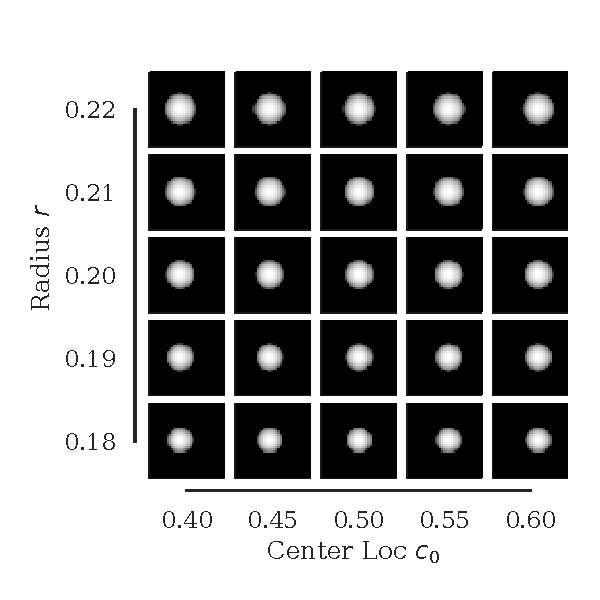
\includegraphics[width=0.9\linewidth]{figs/gasket}
\caption{Gasket profiles depicted as grayscale images simulated with radius
and center location they coincide with on the axes.}
\end{figure}

We define the sources of variation in in-control gasket beads by two
latent variables sampling from independent Gaussian distributions:
\begin{equation}
\begin{split}\czero\sim\Norm(0.5,1\times10^{-2})\\
r\sim\Norm(0.2,6.25\times10^{-4})
\end{split}
\end{equation}

Finally, we will consider the following four types of out-of-control
variation patterns for the system:
\begin{itemize}
\item \textbf{Location shift:} the mean of the process that generates $\czero$
is altered by an amount $\delta$ as in 
\[
\czero\sim\Norm(0.5+\delta\times10^{-2},1\times10^{-2})
\]
\item \textbf{Width shift:} the mean of the process that generates $a$
is perturbed by an amount $\delta$ as in
\[
r\sim\Norm(0.2+\delta\times10^{-4},6.25\times10^{-4})
\]
\item \textbf{Mean shift}: all the pixels are added an additive disturbance
$\delta$ as in 
\[
f(\mbp;c_{0},r)\leftarrow f(\mbp;c_{0},r)+\delta
\]
\item \textbf{Magnitude shift:} all the pixels are added a multiplicative
disturbance $\delta$ as in 
\[
f(\mbp;c_{0},r) \leftarrow f(\mbp;c_{0},r)*\delta
\]
\end{itemize}
Here, $\delta$ is the intensity of the change. Note that the location
shift and width shift represent disturbances in latent distribution
$p_{\delta}(\mbz)$. An important distinction between the two is that
location equivariance is injected into convolutional networks but
not scale equivariance, therefore we expect different reactions to
these changes by deep convolutional latent variable models in terms
of disentanglement. The other two cases, mean shift and magnitude
shift, represent disturbances in the conditional distribution $p_{\delta}(\mbx\g\mbz)$.
The training, validation, and testing in-control or out-of-control
samples are generated of size 500 each.

\subsection{On the Disentanglement and Extrapolation Performance of the Encoder
\label{sec:simstudy:recognition}}

To investigate the disentanglement and extrapolation performance of
the recognition network, we employ the following procedure. First,
we train a VAE with a 2-dimensional latent code (for easier visualization)
to convergence using in-control samples as described in \ref{sec:simsetting}.
Then, we a set of profiles with varying center location $c_{0}$ and
radius $r$ into the recognition network (i.e., encoder network) to
obtain their respective proposal distributions. The points are picked
inside and outside the tolerance region of the two quality characteristics
to be compared against their mapping onto the representation space.
Finally, we sample 150 points from the proposals and plot them on
the representation space. The results are shown in \ref{fig:proposals}
below. There are two important observations we would like to point
out:
\begin{itemize}
\item \textbf{Representations are entangled}. For any of the fixed sources
of variation, the variation in the other source is not axis-parallel
and therefore, the variations are entangled in the learned space.
\item \textbf{The encoder cannot extrapolate for extreme values}.\textbf{
}Observe how for the extremely high values of center location $c$
or extremely low values of radius $r$ are the overall variation pattern
starts getting distorted.
\end{itemize}
Given these two observations and \ref{fig:Fixed-c-varying-r}, we
can conclude right away that gaskets with extremely small radius $r$
will likely go undetected if only the latent variable-based statistic
is used. This is an undesired consequence of the two aforementioned
issues. The model seems to be more accurately responsive to the extreme
values of center location $c$. However, this is most likely due to
translational equivariance injected into the model through convolutional
layers \parencite{locatello2018challenging}. In many real-life applications,
the nature of variations in profiles will be more complex than simple
translations in the spatial or temporal domain. For such variations,
it would be infeasible to inject required predicates due to the rigid
architectures of deep neural networks. We already have the radius
as the evidence because convolutional layers are not scale-equivariant.

\begin{figure}[H]
\subfloat[Fixed $r$, varying $c$\label{fig:Fixed-r-varying-c}]{\centering{}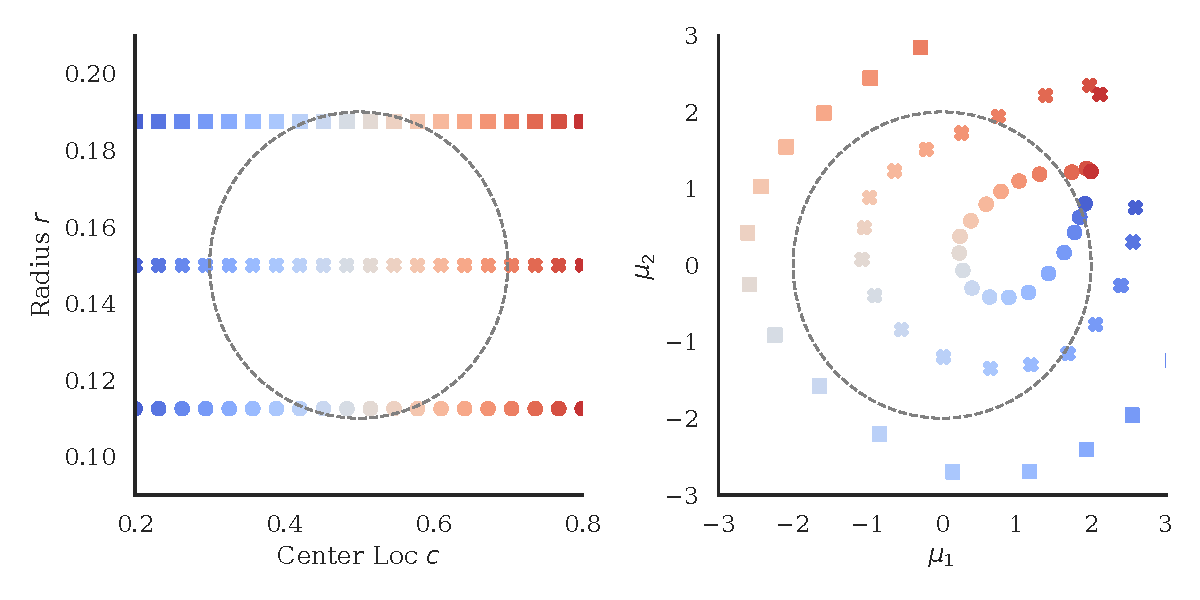
\includegraphics[scale=0.5]{figs/fixed_radii}}

\subfloat[Fixed $c$, varying $r$\label{fig:Fixed-c-varying-r}]{\begin{centering}
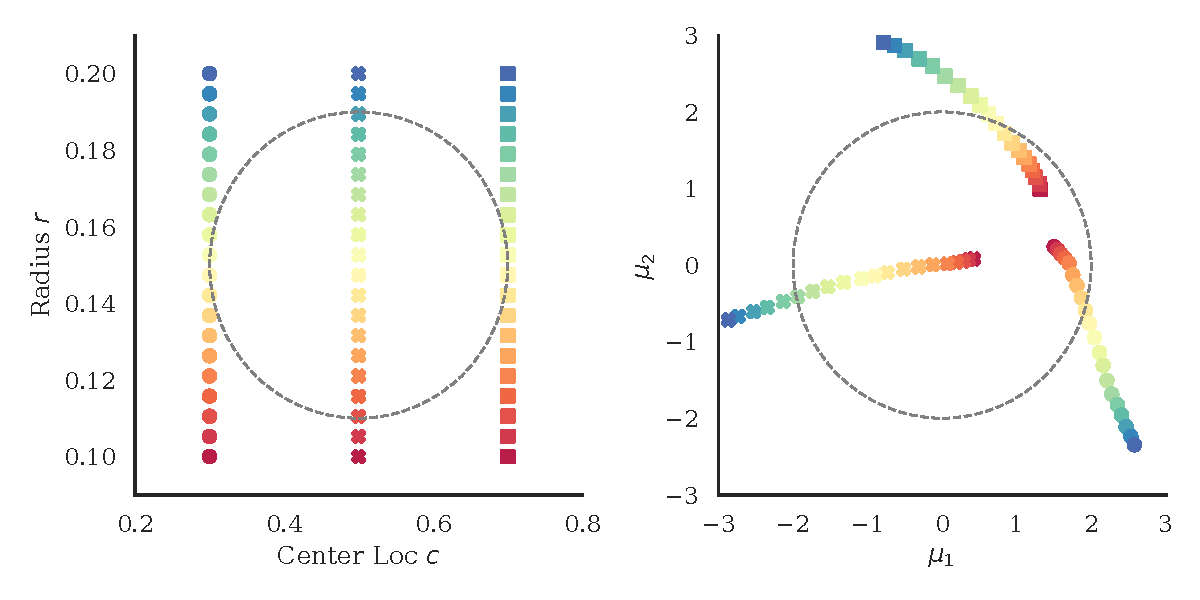
\includegraphics[scale=0.5]{figs/fixed_center_locs}
\par\end{centering}
}\caption{Figure depicting the entangled representations and extrapolation issues
of the encoder of a VAE with two-dimensional latent code trained on
in-control samples with. For each subfigure, plots on the
left show where real factors of variation are sampled from and figure
on the right is what the VAE encoder infers as the mean of the proposal
distribution $\protect\encoding$. \textbf{Top:} Real factors of variation
are generated at three fixed levels of radius $r$ and varying values
of center location $c$ on the left figure. Corresponding inferred
mean plotted on the right graph. \textbf{Bottom:} Similar to (b) but
with fixed center location $c$ at three levels and varying $r$.
The tolerable region is represented by the gray dashed circle, a curve
of isodistant points in terms of Mahalanobis distance to in-control
distribution. Isodistant curve for standard Gaussian that is probability-wise
equivalent to the one on the left is depicted as a gray dashed circle.}
\label{fig:proposals}
\end{figure}

Overall, it is in agreement with our rationale behind the proposed
statistic outlined in \ref{sec:proposed-statistic}. In other words,
without extrapolation and disentanglement, we do not expect any latent-variable-based
monitoring statistic based purely on the output of the recognition
network (such as $H^{2}$, $T^{2}$ or $D$ discussed in \ref{sec:bckgrnd:critique})
to be robust enough to be safely employed in a process control mission.

We also want to make a remark that we tried the beta-VAE framework
explained in \parencite{higgins2017beta} with \textbf{$\beta=4$}
to remedy the problem of entanglement but obtained similar results.
Finding disentangled representations for deep generative models is
still an open research area and to the best of our knowledge, solutions
with theoretical guarantees does not exist.

\subsection{On the Extrapolation Performance of the Decoder \label{sec:simstudy:generator}}

\ref{fig:manifold_vae} hints us about the extrapolation performance
of the decoder of the same VAE described in \ref{sec:simstudy:recognition}
trained on in-control samples described in \ref{sec:simsetting}.
It should be cross-examined with \ref{fig:proposals} above as the
encoder and decoder are tightly coupled to each other. We observe
two important behavior: the posterior gets distorted beyond two or
three standard deviations, and the representations are partially entangled
in line with the behavior of its encoder depicted in \ref{fig:proposals}.
To see how this will help to detect disturbances in latent space,
consider a gasket that is extremely small in terms of the radius (i.e.,
small $r$) or at the very margins of the grid in terms of center
location (i.e., center location $c$ far from 0.5). Looking at \ref{fig:manifold_vae},
we can observe that the decoder simply cannot generate such a sample
because it does not extrapolate well in either of latent dimensions.
This will in turn, produce a larger reconstruction error, and thus
a larger monitoring statistic that will likely to fall outside the
control limit. Recall once again that the disturbance described is
purely on the latent distribution $p_{\delta}(\mbz)$ and yet our
proposed monitoring statistic will capture this behavior well thanks
to the extrapolation issues in the decoder.

\begin{figure}[H]
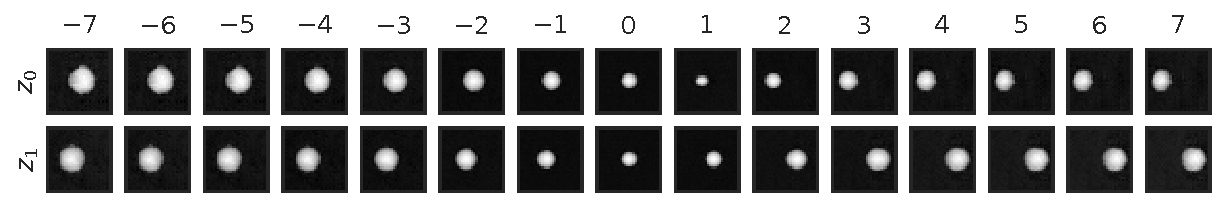
\includegraphics[width=0.9\linewidth]{figs/manifold_vae} \caption{Latent space traversal and the response of the decoder of a VAE with
2-dimensional latent codes and trained with in-control gasket samples.
Each row represents which latent dimension is traversed while the
other dimension is fixed at zero. Each column represents what value
is assigned to that latent dimension that is represented by the row
label. Each image in each cell is generated by the decoder using that
specific latent variable combination.}
\label{fig:manifold_vae}
\end{figure}


\subsection{On the Estimation of Log-likelihood Under Importance Sampling}

Earlier, we claimed that it would take too many Monte Carlo sampling
iterations to get a meaningful estimate of ERE defined as $\E_{\mbz\sim q_{\mbtheta}}\log\decoding$.
In this section, we test that claim on a random in-control sample
$\mbx$ using the proposal distribution $\mbz\sim\encoding$ which
is obtained via the encoder of the same VAE model we have been using
in this section. The results of the sampling-based estimation of ERE,
first-order approximation $ERE_{1}$, and second-order approximation
$ERE_{2}$ are shown in \ref{fig:Estimation-comparison-between} below.
The key observation is that it takes at least a few tens of Monte
Carlo iterations to get a stable and accurate estimation. At that
level, the single pass through the encoder is negligible. This means
using sampling will be more costly at least 50 samples to achieve
the same accuracy as the first-order approximation that we suggest
and at least 80 samples to get the accuracy of the second-order approximation.
Another important observation is that second-order approximation is
a bit more accurate than first-order approximation since it is closer
to the sample average approximation, but their difference is insignificant,
and it requires much more computation. In the next subsection, we
will evaluate the performance of $ERE_{2}$ and $ERE_{1}$ in Phase-II
monitoring to evaluate whether the added computational complexity
for $ERE_{2}$ is justifiable.

\begin{figure}[H]
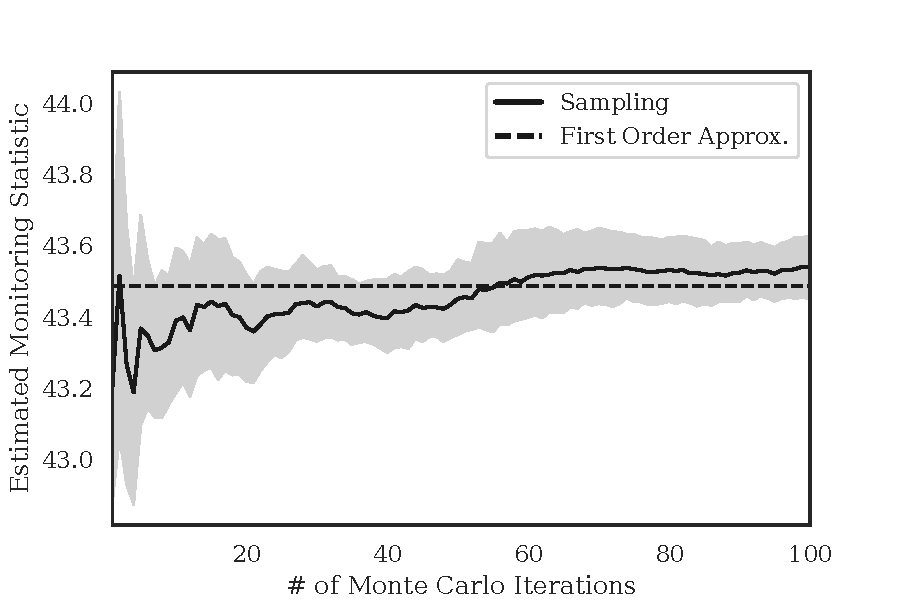
\includegraphics[width=0.9\textwidth]{figs/mc_vs_foa}

\caption{Estimation comparison between Monte Carlo sampling, first-order approximation
and second-order approximation. 95\% confidence interval band is shown
in the gray band and is based on simulations with ten different seeds.
\label{fig:Estimation-comparison-between}}
\end{figure}


\subsection{Comparison of Detection Performance of Proposed Statistics}

We now compare the proposed statistics based on how accurately they
detect profiles from out-of-control processes outlined in \ref{sec:simsetting}.
Note that for all statistics that require sampling, we obtain a single
sample and calculate the statistic based on that to keep the computational
demand the same for all statistics and emulate the computational constraints
of a real-life case. A preliminary result we must check is the robustness
of the statistics by making sure all proposed statistics have false
alarm rates on the held-out in-control test set, which should also
be less than the desired rate 5\%. \ref{tab:far} demonstrates that
this is the case for all of them.

\begin{table}[t]
\global\long\def\arraystretch{1.3}%
 \caption{False alarm rates on the held-out dataset averaged over 10 replications
per model and monitoring statistic. Standard deviations are in parentheses.\label{tab:far}}

\begin{tabular}{llllll}
\toprule 
Statistic & ERE & SPE/R & D & H2 & T2\tabularnewline
 & 0.041(0.006) & 0.051(0.005) & 0.044(0.004) & 0.052(0.005) & 0.043(0.009)\tabularnewline
\bottomrule
\end{tabular}
\end{table}

Through \ref{fig:disturbance_on_pxz}, we observe a clear superiority
of $ERE_{1}$ and $ERE_{2}$ over other methods when the disturbance
is on the observable space (top row). Latent variable-based statistics
$D$, $H^{2}$ and $T^{2}$ fail in this case since that they are
purely computed using the proposal distribution latent variables.
$ERE_{1}$ and $ERE_{2}$ also outperform $SPE/R$, although by a
smaller margin it has with the latent variable-statistics. Between
$ERE_{1}$ and $ERE_{2}$, it's hard to claim which one works better
since their mean performances are quite close to each other.

For the latter two disturbances occurring purely on latent dimensions,
results are presented in the bottom row of \ref{fig:disturbance_on_pxz}.
The key observations can be listed as follows:
\begin{itemize}
\item We observe mixed results but generally $ERE_{1}$ and $ERE_{2}$,
$D$ and $H^{2}$ tend to perform better than $SPE/R$ and $T^{2}$.
A commonality between the former three is that they don't rely on
random samples, supporting our argument against this practice.
\item Observe the radius shift-type disturbance show in the bottom left
figure. Even though $H^{2}$ performs better on positive intensities
(larger radii), it completely misses negative intensities (smaller
radii). We foresaw this result in \ref{sec:simstudy:recognition}.
To reiterate, disentanglement and the lack of extrapolation in the
encoder is the reason behind this. We would also suggest that this
result can extend to all the latent-variable based statistics.
\item Unlike latent variable-based statistics, $ERE_{1}$ and $ERE_{2}$
and $SPE/R$ behave more robustly against varying intensities. In
other words, the detection rate increase with increased intensities
consistently. Among these, we observe that $ERE_{1}$ and $ERE_{2}$
consistently outperform $SPE/R$.
\item $ERE_{1}$ and $ERE_{2}$ perform very similarly. In this case, we
conclude that the second-order information does not help too much
for the Phase-II monitoring. The reason behind this is that the second-order
information also comes from the encoder. However, given that the encoders
is trained on in-control samples and may provide inaccurate information
in the out-of-control regions, the second-order information for out-of-control
samples would be bias. Therefore, it does not provide additional gain
for monitoring performance.
\end{itemize}
\begin{figure}[!t]
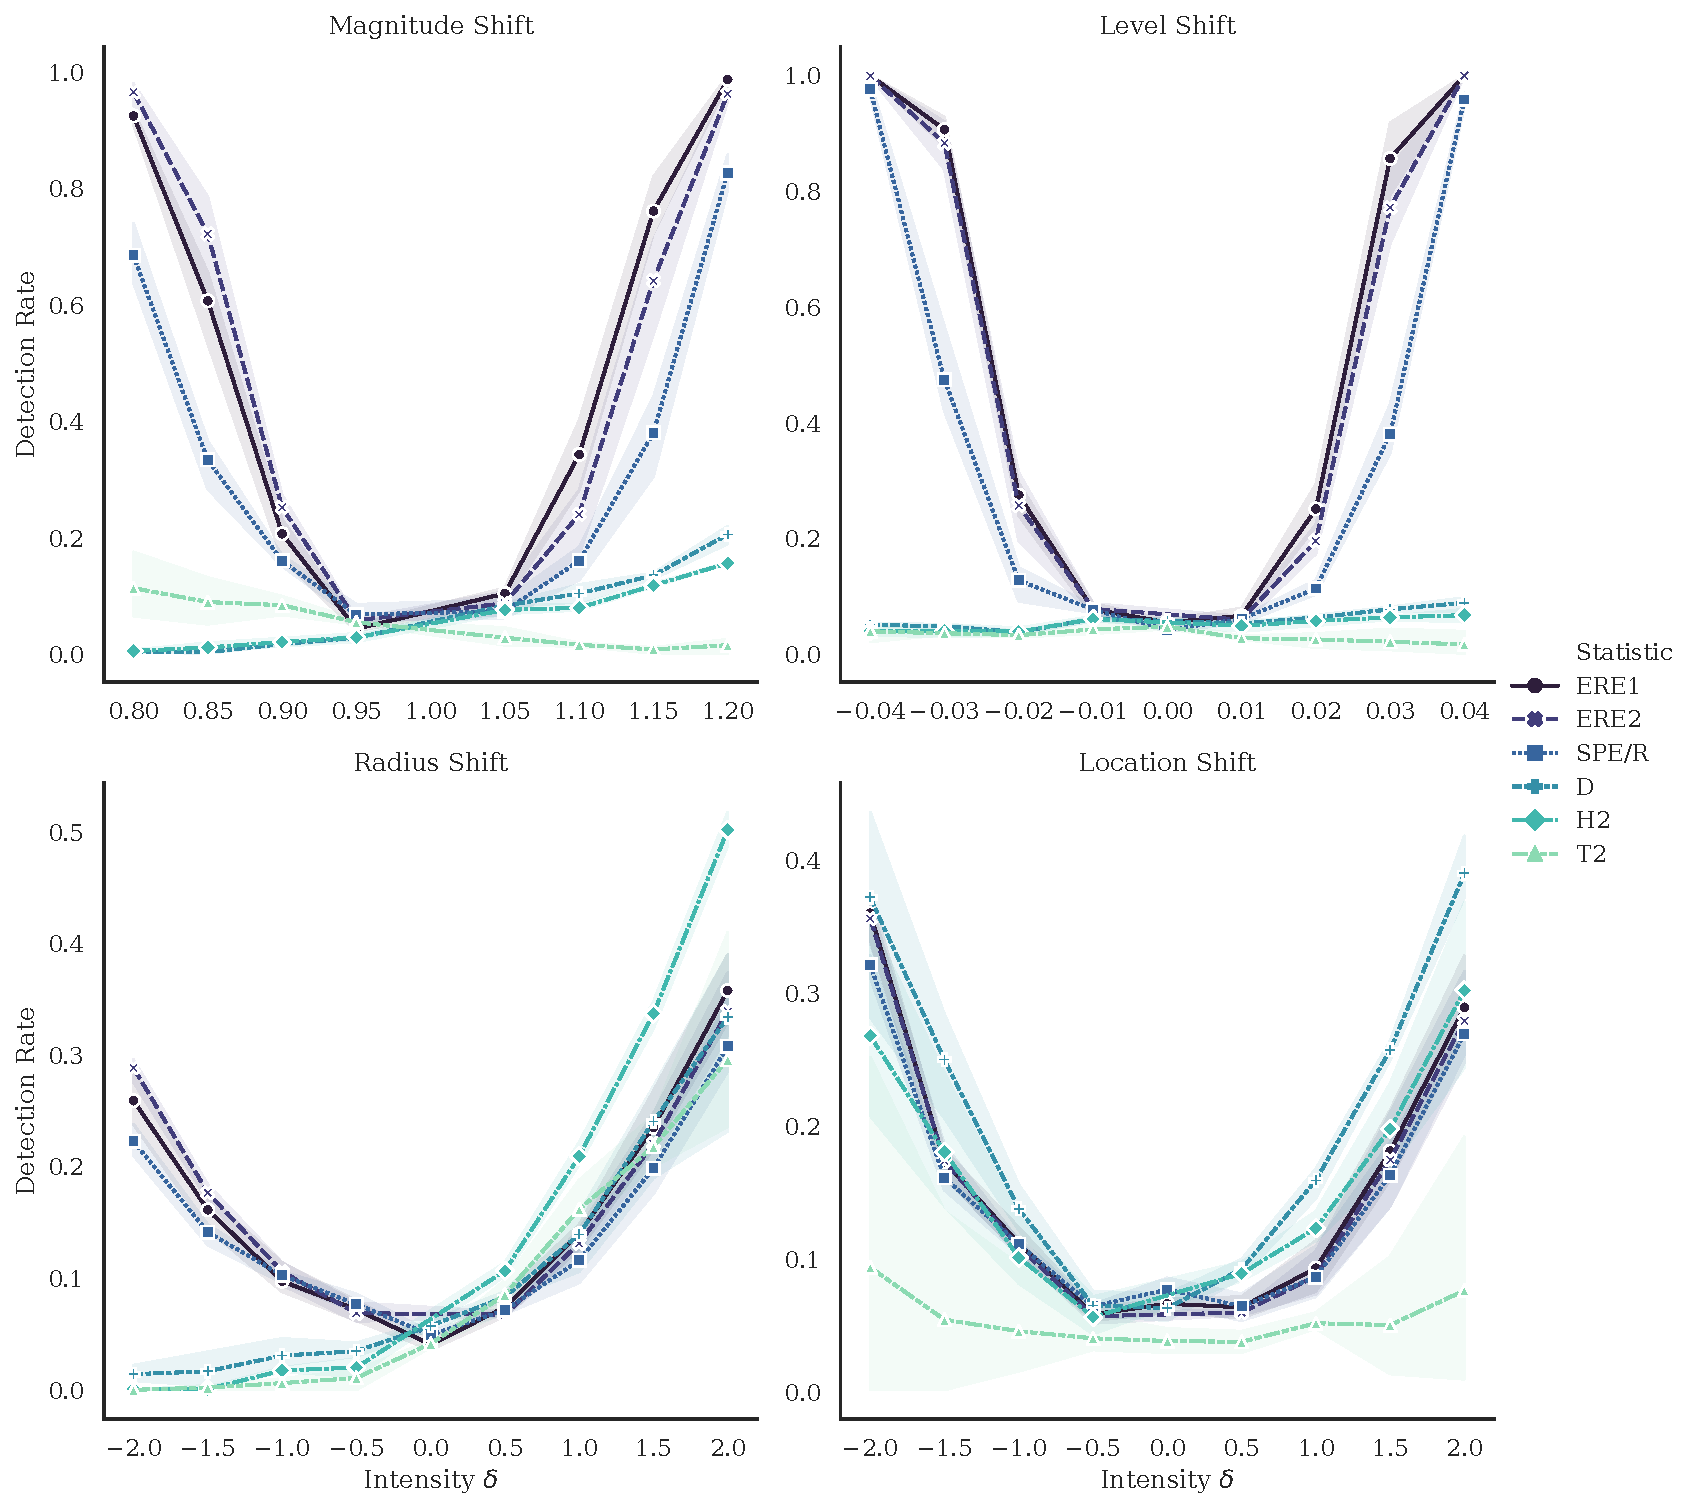
\includegraphics[width=1\linewidth]{figs/disturbance_on_pxz_vae_only}
\caption{Fault detection rates (y-axis) for varying intensities (x-axis) of
different disturbance types (quadrants). Bands represent 95\% confidence
interval estimated around mean detection rates.}
\label{fig:disturbance_on_pxz}
\end{figure}

As mentioned, in a real-life process, disturbances on the residual
space is often more likely than the disturbance in the latent space.
Therefore, we would recommend the use of residual-based monitoring
statistics. Among all residual-based monitoring statistics, we conclude
that $ERE_{1}$ performance the best considering the accuracy, robustness
and computational demand. This will be further validated through the
case study analysis.

\section{Case Study Analysis \& Results}

\label{sec:case-study} % TODO (@DS): how many anomaly samples do we have?
% TODO (@DS): Add a figure to illustrate both normal and abnormal samples, with one image in each class

Our dataset consists of defect image profiles from a hot-steel rolling
process, which is shown in \ref{fig:Rolling}. There are 13 classes
of surface defect types identified by the domain engineers. Four of
these classes---0,1,9 and 11---are considered minor defects and
they constitute our in-control set. There are in total 338 images
in these classes. The other nine classes make up the out-of-control
cases and they have in combination 3351 images to report detection
accuracy for. We randomly partition the in-control corpus to fix train,
validate and test sets with 60\%-20\%-20\% relative sizes, respectively.
The rest of the procedure followed is outlined in \ref{sec:methodology:procedure}.
Same as in the simulation study, to account for randomness in weight
initialization, we replicate the experiment with 10 different seeds.
For comparison, we also include the monitoring performance with the
traditional PCA method with the same residual-based control chart,
denoted as PCA-Q. The results are summarized in \ref{tab:rolling_results}
below.

\begin{sidewaystable}
\global\long\def\arraystretch{1.3}%
 \caption{Summary of fault detection rates on out-of-control cases averaged
over 10 replications per model and monitoring statistic. Standard
deviations are in parentheses. Bolded values represent the maximum
average across different statistics. \label{tab:rolling_results}}

\centering{}%
\begin{tabular}{llllllll}
Model & \multicolumn{6}{c}{VAE} & \multicolumn{1}{c}{PCA}\tabularnewline
Statistic & D & H2 & T2 & SPE/R & ERE & ERE2 & Q\tabularnewline
Fault ID &  &  &  &  &  &  & \tabularnewline
\midrule 
2 & 0.00(0.00) & 0.00(0.00) & 0.00(0.00) & 0.37(0.03) & 0.44(0.06) & \textbf{0.50}(0.06) & 0.00(0.00)\tabularnewline
3 & 0.17(0.06) & 0.23(0.04) & 0.03(0.03) & 0.84(0.01) & 0.85(0.01) & \textbf{0.86}(0.01) & 0.78(0.00)\tabularnewline
4 & 0.00(0.00) & 0.00(0.00) & 0.00(0.00) & 0.62(0.02) & \textbf{0.75}(0.05) & 0.71(0.05) & 0.56(0.00)\tabularnewline
5 & 0.58(0.07) & 0.62(0.09) & 0.00(0.00) & \textbf{1.00}(0.00) & \textbf{1.00}(0.00) & \textbf{1.00}(0.00) & 0.99(0.00)\tabularnewline
6 & 0.06(0.03) & 0.15(0.08) & 0.05(0.05) & 0.79(0.01) & \textbf{0.80}(0.01) & \textbf{0.80}(0.00) & 0.52(0.00)\tabularnewline
7 & 0.01(0.01) & 0.01(0.01) & 0.00(0.00) & 0.13(0.01) & \textbf{0.17}(0.01) & 0.15(0.00) & 0.11(0.00)\tabularnewline
8 & 0.00(0.00) & 0.00(0.00) & 0.00(0.00) & 0.64(0.02) & \textbf{0.70}(0.07) & 0.69(0.01) & 0.34(0.00)\tabularnewline
10 & 0.00(0.00) & 0.00(0.00) & 0.00(0.00) & 0.49(0.03) & \textbf{0.57}(0.05) & \textbf{0.57}(0.04) & 0.29(0.00)\tabularnewline
12 & 0.00(0.00) & 0.00(0.00) & 0.00(0.00) & 0.79(0.01) & \textbf{0.80}(0.02) & \textbf{0.80}(0.02) & 0.69(0.00)\tabularnewline
13 & 0.00(0.00) & 0.00(0.00) & 0.01(0.00) & 0.71(0.04) & \textbf{0.77}(0.02) & 0.76(0.02) & 0.56(0.00)\tabularnewline
\bottomrule
\end{tabular}
\end{sidewaystable}

From \ref{tab:rolling_results}, we can observe that $ERE_{1}$ and
$ERE_{2}$ consistently outperforms all other monitoring statistic
formulations. The divide between residual-based statistics and latent
variable-based statistics observed in the simulation study is further
validated here too. The inferiority of latent variable-based statistics
are much more obvious here in the real case study, as we observe for
most out-of-control classes the detection rate is simply zero. This
observation further validates our claims that in practice, for deep
autoencoders, the change happens in the residual space rather than
the latent space. The advantage of VAE over PCA is mainly due to the
better representative power and data compression ability of deep autoencoders
compared to PCA. It is worth noting that the superiority of VAE over
PCA for process monitoring was also demonstrated in the earlier works
in various applications \parencite{Zhang2019-lu,wang2019systematic,lee2019process}.

To support our claim of the ineffectiveness of latent variable-based
statistics, we refer the reader to \ref{fig:kde} below. We observe
how well separated the statistics are for $ERE_{1}$ and $SPE/R$
while for latent variable-based statistics the obtained values are
mostly overlapping. Note that we omitted $ERE_{2}$ because it was
almost identical to $ERE_{1}$. To obtain a deeper understanding of
the results, we point out in \ref{fig:Output-of-the} for the original
images and their reconstructions. The decoder is persistent on generating
samples that look like in-control rolling samples with little fidelity
to how the original defect sample looks like. When \ref{fig:Original-profiles}
and \ref{fig:Reconstructions-via-VAE} are cross-examined, it is apparent
why reconstruction error would be high. On the contrary, \ref{fig:Inferred-means}
shows that most latent representations fall into the region that would
be considered in-control from a profile monitoring perspective. We
observe instances of class 3,5,6 and 7 generate the latent variables
in the out-of-control regions. However, even for these classes, $SPE/R$,
$ERE_{1}$ and $ERE_{2}$ yields much better detection power than
$D$, $H_{2}$, and $T_{2}$, as it can be seen in \ref{tab:rolling_results}.
In conclusion, we would like to suggest the use of $ERE_{1}$ for
deep autoencoders, which is consistent with our findings in the simulation
study.

\begin{figure}[H]
\begin{subfigure}[b]{0.3\textwidth}
     \centering
     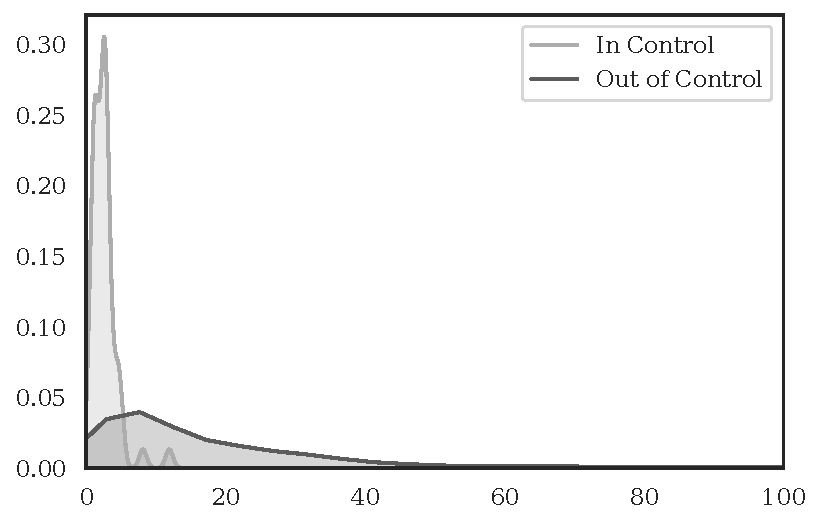
\includegraphics[width=\textwidth]{figs/kdes/SPE.pdf}
     \caption{$ERE_{1}$}
     \label{fig:kde:ERE}
 \end{subfigure}
 \hspace{0.1\textwidth}
 \begin{subfigure}[b]{0.3\textwidth}
     \centering
     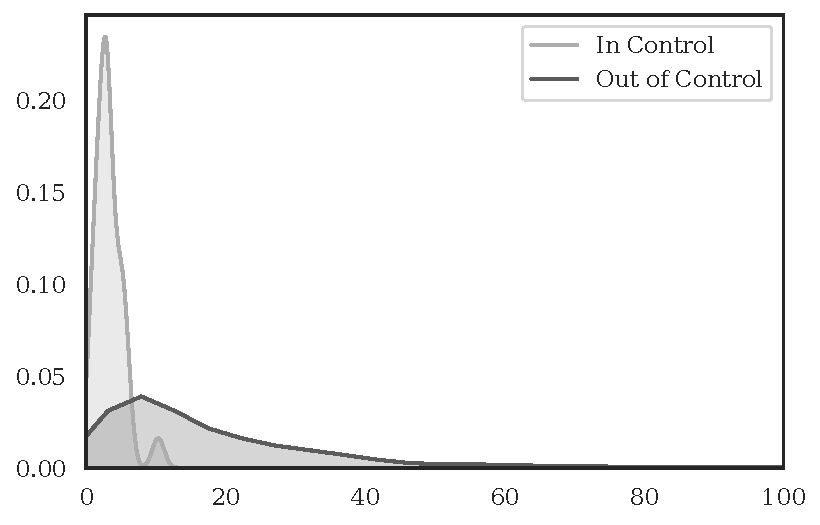
\includegraphics[width=\textwidth]{figs/kdes/R.pdf}
     \caption{$SPE/R$}
     \label{fig:kde:spe-r}
 \end{subfigure}
 
\begin{subfigure}[b]{0.3\textwidth}
     \centering
     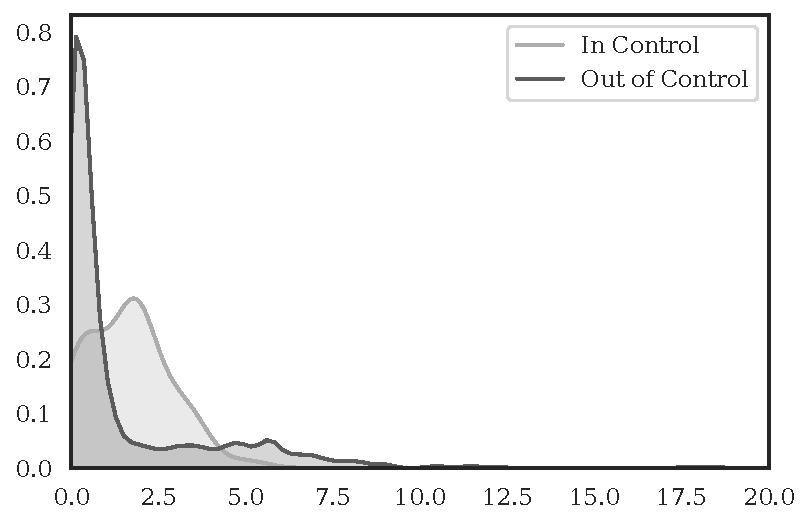
\includegraphics[width=\textwidth]{figs/kdes/H2.pdf}
     \caption{$H^{2}$}
     \label{fig:kde:h2}
\end{subfigure}
\hfill
\begin{subfigure}[b]{0.3\textwidth}
     \centering
     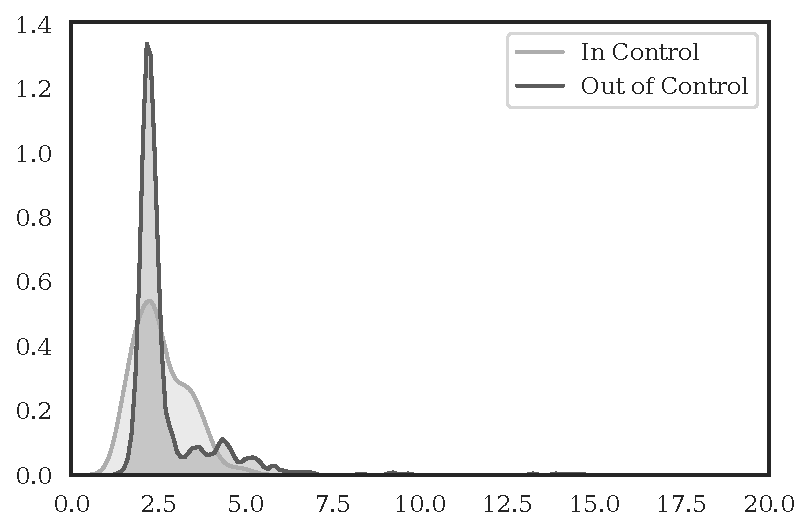
\includegraphics[width=\textwidth]{figs/kdes/D.pdf}
     \caption{$D$}
     \label{fig:kde:D}
\end{subfigure}
\hfill
\begin{subfigure}[b]{0.3\textwidth}
     \centering
     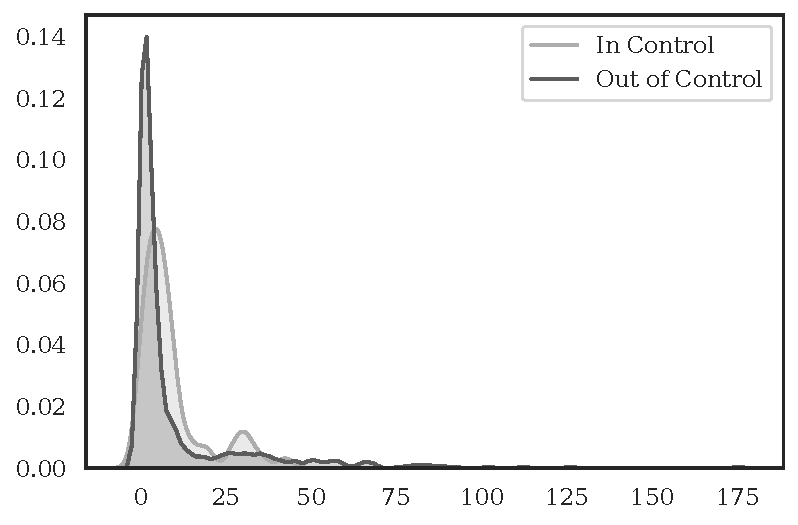
\includegraphics[width=\textwidth]{figs/kdes/T2.pdf}
     \caption{$T^{2}$}
     \label{fig:kde:T2}
\end{subfigure}

\caption{Kernel density estimation plots of statistics obtained for in-control
and out-of-control steel defect profiles, per each proposed statistic
type.\label{fig:kde}}
\end{figure}

\begin{figure}[H]
\begin{minipage}[t]{0.25\textwidth}%
\subfloat[Original profiles\label{fig:Original-profiles}]{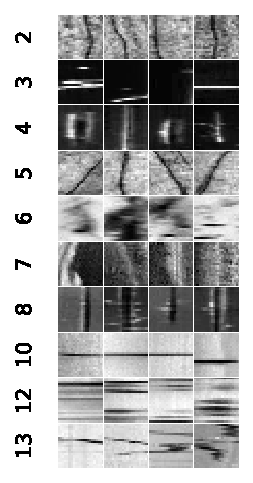
\includegraphics[width=0.99\textwidth]{figs/casestudy_orig}}%
\end{minipage}\hfill{}%
\begin{minipage}[t]{0.25\textwidth}%
\subfloat[Reconstructions via VAE\label{fig:Reconstructions-via-VAE}]{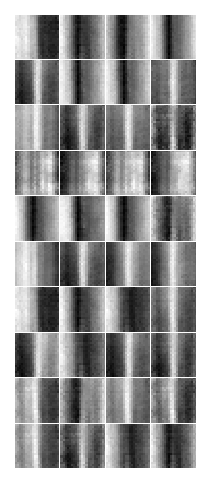
\includegraphics[width=0.82\columnwidth]{figs/casestudy_recons}
}%
\end{minipage}\hfill{}%
\begin{minipage}[t]{0.45\textwidth}%
\subfloat[Inferred means\label{fig:Inferred-means}]{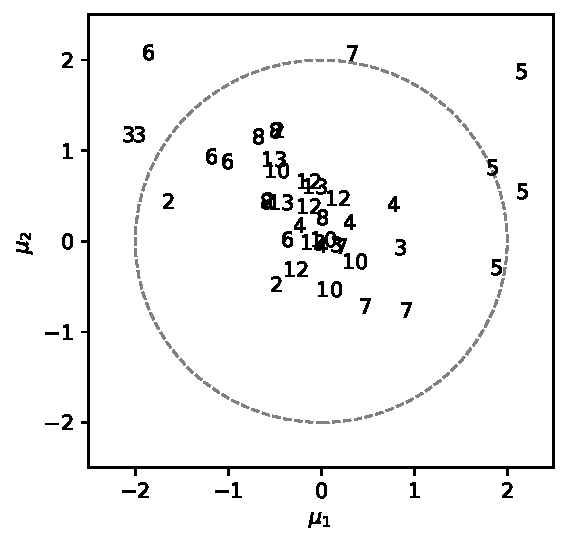
\includegraphics[width=1\textwidth]{figs/casestudy_scat}

}%
\end{minipage}\caption{Output of the VAE decoder and the encoder for randomly select rolling
profiles. \textbf{Left: }Original profiles visualized. Each row is
a class of defect profile and each column is a randomly selected from
that class. \textbf{Middle: }Reconstructions of the samples with one-to-one
correspondence to the samples on the image to the left. \textbf{Right:
}Inferred mean locations of each of the defects visualized on left.
Points are annotated by their class IDs. \label{fig:Output-of-the}}
\end{figure}


\section{Conclusion \label{sec:conclusions}}

In this paper, we focused on evaluating Phase-II monitoring statistics
proposed so far in the literature for VAE and demonstrate that they
were not performing optimally in terms of accuracy and/or computational
feasibility. First, we classified the monitoring statistics for latent-variable-based and residual-based and show how these are natural extension of monitoring statistics for PCA.
Second, we further pointed out two important issues related to the
latent variables learned by the encoder of VAE, namely, entanglement
and failure to extrapolate. Based on these issues, unlike PCA, we demonstrated that latent
variable-based statistics should be discarded altogether with both
conceptual explanations and real experiments. Third, we pointed out
that the residual-based statistics based on sampling will require
too many samples to be computationally feasible. Finally, we proposed
a novel formulation by deriving the Taylor expansion of expected reconstruction
error that addresses both accuracy and computational efficiency.

To support our claim, our simulation study first demonstrated the
entanglement and lack of extrapolation of latent variable-based statistics
and its inferior Phase-II monitoring performance. It further showed
that the derived statistics based on the residual space is more robust
and more accurate than all the other statistics proposed so far. Finally,
we validated the superiority of our formulation on a real-life case
study, where steel defect image profiles are used.

\printbibliography


\appendix
%dummy  inserted by tex2lyx to ensure that this paragraph is not empty\refalias{section}{appendix}

\section{Proof of Proposition 3.1 \label{sec:PoofOfPropTQ}}

The Kullback-Leibler divergence between two multivariate Gaussian
distributions has a closed-form solution. If we define these distributions
as $p_{0}=N(\mbz;\mbmu_{0},\mbSigma_{0})$ and $p_{1}=N(\mbz;\mbmu_{1},\mbSigma_{1})$
where $\mbmu$ and $\mbSigma$ are respective mean vectors and covariance
matrices, then according to \textcite{hershey2007approximating}
the closed-form solution will be the following: 
\begin{align}
\KL{p_{0}}{p_{1}} & =\frac{1}{2}[\log\frac{\g\mbSigma_{1}\g}{\g\mbSigma_{0}\g}+Tr(\mbSigma_{1}\inv\mbSigma_{0})-r+(\mbmu_{0}-\mbmu_{1})^{\top}\mbSigma_{1}\inv(\mbmu_{0}-\mbmu_{1})]\label{eq:kld-closed-form}
\end{align}
Since $\encoding=\Norm(\mbmu(\mbx),\mbSigma_{z})$ and $p(\mbz)=\Norm(0,\mbI)$,
we can derive that 
\begin{align}
\KL{\encoding}{p(\mbz)} & =\frac{1}{2}\left[-\log\g\mbSigma_{z}\g+Tr(\mbSigma_{z})-r\right]+\frac{1}{2}\mbmu(\mbx)^{\top}\mbmu(\mbx)\nonumber \\
 & =\frac{1}{2}\mbmu(\mbx)^{\top}\mbmu(\mbx)+C,\label{eq:kld-prior}
\end{align}
where $C=-\log\g\mbSigma_{z}\g+Tr(\mbSigma_{z})-r$ is a constant,
which doesn't depend on $\mbx$.

To derive the SPE statistics, we will derive

\begin{align}
 & \mathbb{E}_{\mbz\sim q_{\mbtheta}}\|\mbx-\mbW\mbz\|^{2}\nonumber \\
= & \mathbb{E}_{\mbz\sim q_{\mbtheta}}(\mbx^{\top}\mbx-2\mbz^{\top}\mbW\mbx+\mbz^{\top}\mbW^{\top}\mbW\mbz)\nonumber \\
= & \mbx^{\top}\mbx-2\mbmu(\mbx)^{\top}\mbW\mbx+\mathbb{E}_{\mbz\sim q_{\mbtheta}}(\mbz^{\top}\mbW^{\top}\mbW\mbz)\label{eq: spew}
\end{align}

Here, we know that 
\begin{align}
 & \mathbb{E}_{\mbz\sim q_{\mbtheta}}(\mbz^{\top}\mbW^{\top}\mbW\mbz)\nonumber \\
= & \mathbb{E}_{\mbz\sim q_{\mbtheta}}tr(\mbz^{\top}\mbW^{\top}\mbW\mbz)\nonumber \\
= & tr\left(\mbW^{\top}\mbW\mathbb{E}_{\mbz\sim q_{\mbtheta}}(\mbz\mbz^{\top})\right)\nonumber \\
= & tr\left(\mbW^{\top}\mbW(\mbmu(\mbx)\mbmu(\mbx)^{\top}+\Sigma_{z})\right)\nonumber \\
= & \mbmu(\mbx)^{\top}\mbW^{\top}\mbW\mbmu(\mbx)+tr\left(\mbW^{\top}\mbW\Sigma_{z}\right)\label{eq: tracezwwz}
\end{align}

Therefore, by plugging \ref{eq: tracezwwz} into \ref{eq: spew},
we have 
\begin{align}
\mathbb{E}_{\mbz\sim q_{\mbtheta}}\|\mbx-\mbW\mbz\|^{2} & =\mbx^{\top}\mbx-2\mbmu(\mbx)^{\top}\mbW\mbx+\mathbb{E}_{\mbz\sim q_{\mbtheta}}(\mbz^{\top}\mbW^{\top}\mbW\mbz)\nonumber \\
 & =\mbx^{\top}\mbx-2\mbmu(\mbx)^{\top}\mbW\mbx+\mbmu(\mbx)^{\top}\mbW^{\top}\mbW\mbmu(\mbx)+tr\left(\mbW^{\top}\mbW\Sigma_{z}\right)\nonumber \\
 & =\|\mbx-\mbW\mbmu(\mbx)\|^{2}+C\label{eq:q-to-ere}
\end{align}
where $C=tr\left(\mbW^{\top}\mbW\Sigma_{z}\right)$ that does not
depend on $\mbx$.

\section{A Toy Example to Demonstrate Out-of-distribution Behavior of Neural
Networks \label{app:rosenbrock}}

Assume using a multilayer perceptron, we are trying to approximate
the famous Rosenbrock function $f(x,y)=(a-x)^{2}+b(y-x^{2})^{2}$
given $(a,b)=(1,100)$. In this small experiment, we sample tuples
of two-dimensional points from a bounded region $(x_{i},y_{i})\in[-1,3]\times[-2,3]$.
We use a multilayer perceptron with six hidden layers and a hundred
neurons in each layer. Half of the points are used in training, and
the other half is used as a validation set to optimize hyper-parameters.
Using the trained network, we plot the actual Rosenbrock function
along with the neural network approximation in \ref{fig:Rosenbrock}.
Notice how well the function is approximated for the region $[-1,3]\times[-2,3]$,
but there is a serious discrepancy between the approximated and the
real outside of the region. This is a small yet to the point example
of out-of-distribution issues with neural networks.

\begin{figure}
\begin{centering}
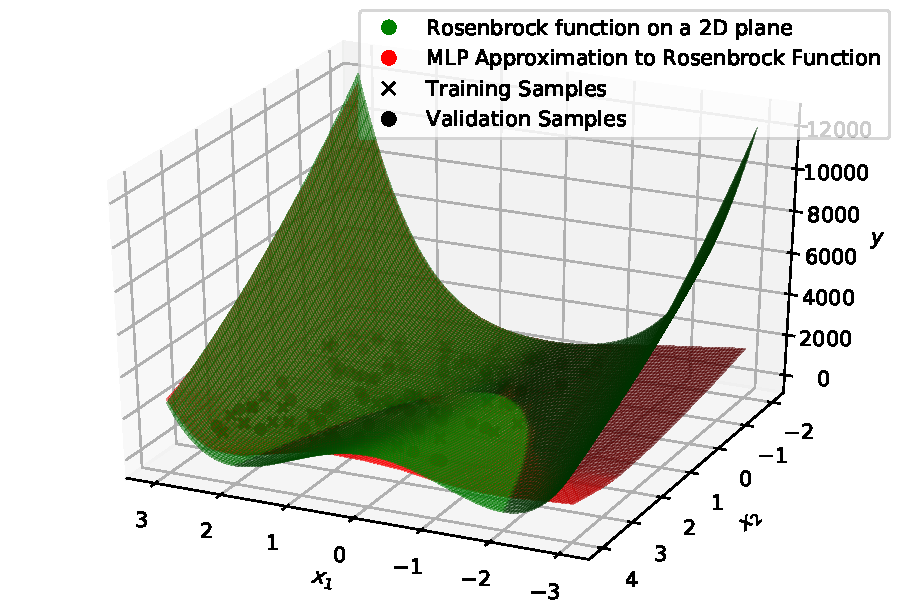
\includegraphics[width=1\textwidth]{figs/rosenbrock}
\par\end{centering}
\caption{Rosenbrock function (green surface) approximated by an multilayer
perceptron(red surface) given training (black crosses) and validation
(black dots) samples form a bounded region $(x_{i},y_{i})\in[-1,3]\times[-2,3]$.\label{fig:Rosenbrock}}
\end{figure}


\section{ERE Testing Statistic Derivation \label{app:ere}}

To derive the $ERE_{1}$ and $ERE_{2}$, we first define $R(z)=\|y-\mbmu_{\mbtheta}(z)\|^{2}$
as the reconstruction error (RE). The quantity we would like approximate
is $E_{\mbz\sim q_{\phi}}R(\mbz)$ where $\encoding=\Norm(\mbmu_{\mbphi}(\mbx),\Sigma_{z})$.
We are looking for the Taylor expansion of the expected RE (ERE) around
$z_{0}=\mbmu_{\mbphi}(\mbx)$, i.e., the first moment. For notational
simplicity, we use $H_{z}$ to denote the Hessian $R''(\mbmu_{\mbphi}(\mbx))$.
The derivation is formalized as follows:

\begin{align}
E_{\mbz\sim q_{\phi}}R(\mbz) & =R(\mbmu_{\mbphi}(\mbx))+R'(\mbmu_{\mbphi}(\mbx))E_{\mbz\sim q_{\phi}}[\mbz-\mbmu_{\mbphi}(\mbx)])\nonumber \\
 & \quad+\frac{1}{2}E_{\mbz\sim q_{\phi}}[(\mbz-\mbmu_{\mbphi}(\mbx))^{\top}\mathbf{H}_{z}(\mbz-\mbmu_{\mbphi}(\mbx))]+O(\|(\mbz-\mbmu_{\mbphi}(\mbx)\|^{3}\nonumber \\
 & \simeq R(\mbmu_{\mbphi}(\mbx))+\frac{1}{2}E_{\mbz\sim q_{\phi}}[(\mbz-\mbmu_{\mbphi}(\mbx))^{\top}\mathbf{H}_{z}(\mbz-\mbmu_{\mbphi}(\mbx))]\nonumber \\
 & =R(\mbmu_{\mbphi}(\mbx))+\frac{1}{2}\mathrm{tr}(\mathbf{H}_{z}E[(\mbz-\mbmu_{z})(\mbz-\mbmu_{z})^{T}])\nonumber \\
 & =R(\mbmu_{\mbphi}(\mbx))+\frac{1}{2}\mathrm{tr}(\mathbf{H}_{z}\Sigma_{z})\label{eq:derived-ere2}
\end{align}

Note for $ERE_{1}$, the second term $\frac{1}{2}\mathrm{tr}(\mathbf{H}_{z}\Sigma_{z})$
is droped and we are left with $R(\mbmu_{\mbphi}(\mbx))$ only. For $ERE_{2}$,
since $\Sigma_{z}$ is a diagonal matrix, $\mathrm{tr}(\mathbf{H}_{z}S_{z})=\mathrm{tr}(diag(\mathbf{H}_{z})S_{z})=\sum_{i}(\mathbf{H}_{z})_{ii}(S_{z})_{ii}$
holds. We can utilize this result to compute $ERE_{2}$, in a more computationally
efficient manner.
\end{document}
